\documentclass[12pt]{report}
\usepackage{psfig,setspace}
\usepackage{pslatex}
\usepackage[a4paper,left=1.5in,right=1in,top=1.5in]{geometry}
\usepackage[intlimits]{amsmath}
\usepackage{paralist}
\usepackage{makeidx}
\usepackage{graphicx,amssymb,amsthm}
\usepackage{amsmath, amssymb, amsthm}
\usepackage{hyperref}
%\usepackage[ruled,linesnumbered,algosection]{algorithm2e}
\usepackage{appendix}
%\usepackage{subfig,multirow,longtable,fancyhdr,figsize,multicol}
\usepackage{multirow}
\usepackage{multicol}
\usepackage{subfig} 
\usepackage{fancyhdr}
\usepackage{pslatex}
\usepackage{epsfig}
\usepackage{ulem}
\usepackage[T1]{fontenc} 
%\usepackage{algorithmic}
\usepackage{algorithm}
\usepackage{float}
\usepackage{slashbox}
\usepackage{marvosym}
\usepackage[section] {placeins}
\usepackage{morefloats}
\usepackage{algcompatible}
\usepackage{booktabs}
\usepackage{comment}
\usepackage{caption}
\usepackage[nottoc]{tocbibind}
% ,numbib

\newtheorem{lemma1}{Lemma}
\newtheorem{lemma2}[lemma1]{Lemma}
\newtheorem{definition1}{Definition}
\newtheorem{definition2}[definition1]{Definition}
\newtheorem{definition3}[definition1]{Definition}
\newtheorem{definition4}[definition1]{Definition}

\linespread{1.5}
\normalem
\newtheorem{mydef}{Definition}
\setlength{\headheight}{16pt}
\newcommand{\secref}[1]{Section~\ref{#1}}
\newcommand{\NI}{\noindent}
\newcommand{\midplusspace}{\baselineskip0.26truein}
\setcounter{secnumdepth}{4} \setcounter{tocdepth}{4}


\begin{document}
\pagenumbering{roman}
\setcounter{page}{1}
\thispagestyle{empty}
\vspace{1cm}

\begin{center}
%	\pagestyle{myheadings}
% 	\textbf { \LARGE Spatial Data: Crawling, Metadata Discovery, Publishing \& Query Orchestration}
	\textbf { \LARGE SPATIAL DATA: CRAWLING, METADATA DISCOVERY, PUBLISHING \& QUERY ORCHESTRATION}
	%\vspace*{0.1cm}
	%\textbf { \LARGE Separation of Duty Constraints}
	\vspace{1.7in}

	{\bf Punjabi Deepak Bharatbhai }\\
	{\bf Roll No. 15IT60R17}\\
	  \vspace{1.2 in}
	  \begin{figure}[h]
	    \centering
	   %   
\includegraphics[height=1.4in,width=1.2in]{images/IITLogo.jpg}
	        
\includegraphics[scale=0.15]{images/logo.png}
	    \end{figure}
	 \begin{center}
	    {{\bf DEPARTMENT OF COMPUTER SCIENCE AND ENGINEERING } \\
	        {\bf INDIAN INSTITUTE OF TECHNOLOGY, KHARAGPUR}\\
	        {\bf WEST BENGAL, INDIA}\\ 
		 {\bf APRIL 2017}
	    }
	  \end{center}
\end{center}

%   \pagebreak
     \clearpage
     \newpage
     \thispagestyle{empty}
     \mbox{}
     \newpage

\newpage
\date{}
\thispagestyle{empty}

% Page 1 : Main Text
\thispagestyle{empty}
\begin{center}
% \textbf{\large Area Sweep Coverage in Wireless Sensor Networks }
\textbf{ \LARGE{SPATIAL DATA: CRAWLING, METADATA DISCOVERY, PUBLISHING \& QUERY ORCHESTRATION} }
\end{center}
 \vspace{-2.5em}
\begin{center}
% \textbf{Geo-Service Portal -- Foundation Platform}
\end{center}
 \vspace{-2.5em}
\begin{center}
\textbf{\large Geo - Service Portal }\\
% \textbf{ Foundation Platform }
\end{center}
% Uncomment the following if a third line is required
%  \vspace{-2.5em}
% \begin{center}
%  \textbf{\large FOLLOWED BY THE THIRD ONE}
% \end{center}
 \vspace{2em}
\begin{center}
 \textbf{\textit{Thesis submitted to Indian Institute of Technology Kharagpur}} 
\end{center}
 \vspace{-3em}
\begin{center}
 \textbf{\textit{in partial fulfillment of the requirements for the award of the }} 
\end{center}
 \vspace{-3em}
\begin{center}
 \textbf{\textit{degree of}}
\end{center}
 \vspace{-1em}
\begin{center}
 \textbf{ Master of Technology}
\end{center}
\vspace{-3em}
\begin{center}
 \textbf{\textit{in}}
\end{center}
 \vspace{-3em}
\begin{center}
 \textbf{{Information Technology}}
\end{center}
 \vspace{-3em}
\begin{center}
 \textit{by}
\end{center}
 \vspace{-1em}
\begin{center}
 \large{\textbf{Punjabi Deepak Bharatbhai}}
\end{center}
 \vspace{-3em}
\begin{center}
 \large{\textbf{15IT60R17}}
\end{center}
 \vspace{-1em}
\begin{center}
 Under the guidance of
\end{center}
 \vspace{-2.5em}
\begin{center}
 \large \textbf{Prof. Soumya K. Ghosh}
\end{center}
 \vspace{0em}
\begin{center}

\includegraphics[scale=0.15]{images/logo.png}
\end{center}
 \vspace{-1em}
\begin{center}
 \textbf{\small DEPARTMENT OF COMPUTER SCIENCE AND ENGINEERING}
\end{center}
 \vspace{-3em}
\begin{center}
 \textbf{\small INDIAN INSTITUTE OF TECHNOLOGY KHARAGPUR} 
\end{center}
 \vspace{-3em}
\begin{center}
 \textbf{\small APRIL 2017}
\end{center}
 \vspace{-1em}
\begin{center}
 \copyright 2017 Deepak Punjabi. All rights reserved.
\end{center}

\clearpage
%\newpage
%\thispagestyle{empty}
%\cleardoublepage

\newpage

% \thispagestyle{empty}
\vspace{1cm}
\begin{center}
\vspace*{0.1cm}
\textbf { \LARGE  Rumor Detection in Online Social Networks}
%\vspace*{0.1cm}
%\textbf { \LARGE Cardinality Constraints}
\vskip 0.2in
\large {\textbf { {A Thesis submitted in  partial fulfilment of the}}}
\vskip .01in
\large {{\textbf {requirements for the degree of}}}
\vskip .1in
\textbf{\Large Master of Technology}
\vskip .05in
\centerline{\textbf{in}}
\vskip .05in
\centerline{\textbf{\Large{Information Technology}}}
\vskip .05in
\textbf{\large {\textit by}}
\vskip .05in
\textbf{\Large {Kale Ashish Anil}}
\vskip .05in
\textbf{\large{Roll No. 14IT60R03}}
\vskip .05in
\large {under the supervision of}
\vskip .05in
\textbf{\Large Prof. Shamik Sural}
\vskip .05in
\begin{figure}[h]
\centering

\includegraphics[height=1.4in,width=1.2in]{images/IITLogo.jpg}
\end{figure}
\vskip .05in
\textbf{\large Department of Computer Science \& Engineering}
\vskip .1in
\textbf{\large Indian Institute of Technology, Kharagpur}
\vskip .1in
\textbf{\large West Bengal, India}
\vskip .05in
\textbf{\large April 2016}
\end{center}

%   \pagebreak
     \clearpage
     \newpage
     \thispagestyle{empty}
     \mbox{}
     \newpage

%\newpage 
\addcontentsline{toc}{chapter}{\numberline{}Declaration}
\begin{spacing}{1.07}
\begin{center}
\vspace*{0.1cm}
\vskip 0.1in
\textbf{ \Large \underline{DECLARATION}}
\vskip 0.05in
\vskip 0.1in
\vskip 0.2in
\end{center}
\vskip 0.1in
I, \textbf{Punjabi Deepak Bharatbhai}, Roll No.\textbf{15IT60R17}, registered as a student of M.Tech. program in the Department of Computer Science \& Engineering, Indian Institute of Technology, Kharagpur, India (hereinafter referred to as the 'Institute') do hereby submit my thesis, title: \textbf{Spatial Data: Crawling, Metadata Discovery, Publishing \& Query Orchestration} (hereinafter referred to as 'my thesis') in a printed as well as in an electronic version for holding in the library of record of the Institute.
\vskip 0.1in
\begin{flushleft}
I hereby declare that:
\end{flushleft}
\hspace*{0.6cm}1. The electronic version of my thesis submitted herewith on CDROM is in PDF format.
\vskip 0.1in
2. My thesis is my original work of which the copyright vests in me and my thesis does not infringe or violate the rights of anyone else.\vskip 0.1in
3. The contents of the electronic version of my thesis submitted herewith are the same as that submitted as final hard copy of my thesis after my viva voice and adjudication of my thesis on 03-05-2017.\vskip 0.1in
4. I agree to abide by the terms and conditions of the Institute Policy on Intellectual Property (hereinafter 'Policy') currently in effect, as approved by the competent authority of Institute.\vskip 0.1in
5. I agree to allow the Institute to make available the abstract of my thesis in both hard copy (printed) and electronic form.
\vskip 0.1in6. For the Institute's own, non-commercial, academic use I grant to the Institute the non-exclusive license to make limited copies of my thesis in whole or in part and to loan such copies at the Institute's discretion to academic persons and bodies approved of from time to time by the Institute for non-commercial academic use. All usage under this clause will be governed by the relevant fair use provisions in the Policy and by the Indian Copyright Act in force at the time of submission of the thesis.
\vskip 0.1in7. Furthermore\newline
\hspace*{1.7cm}(a) I agree to allow the Institute to place such copies of the electronic version of my  thesis on the private Intra-net maintained by the Institute for its own academic community.\newline
\hspace*{1.7cm}(b) I agree to allow the Institute to publish such copies of the electronic version of my thesis on a public access website of the Internet should it so desire.
\vskip 0.1in8. That in keeping with the said Policy of the Institute I agree to assign to the Institute (or its Designee/s) according to the following categories all rights in inventions, discoveries or rights of patent and/or similar property rights derived from my thesis where my thesis has been completed:\vskip 0.1in
\hspace*{1cm}a. with use of Institute-supported resources as defined by the Policy and revisions thereof,\newline
\hspace*{1.6cm}b. with support, in part or whole, from a sponsored project or program, vide clause 6(m) of the Policy.\newline \newline
\hspace*{1.1cm}I further recognize that:\vskip 0.05in
\hspace*{1cm}c. All rights in intellectual property described in my thesis where my work does not qualify under sub-clauses 8(a) and/or 8(b) remain with me.
\vskip 0.1in9. The Institute will evaluate my thesis under clause 6(b1) of the Policy. If intellectual property described in my thesis qualifies under clause 6(b1) (ii) as Institute-owned intellectual property, the Institute will proceed for commercialization of the property under clause 6(b4) of the Policy. I agree to maintain confidentiality as per clause 6(b4) of Policy.
\vskip 0.1in10. If the Institute does not wish to file a patent based on my thesis, and it is my opinion that my thesis describes patentable intellectual property to which I wish to restrict access, I agree to notify the Institute to that effect. In such a case no part of my thesis may be disclosed by the Institute to any person(s) without my written authorization for one year after the date of submission of the thesis or the period necessary for sealing the patent, whichever is earlier.
%\vskip 1in
\newline
\vspace{1cm} \hfill
\begin{flushright}
\begin{tabular}{l} \tabularnewline
\hline
Punjabi Deepak Bharatbhai
\tabularnewline
\end{tabular}\\
\hspace{3cm} Department of Computer Science \& Engineering,\\
\hspace{3cm} Indian Institute of Technology, Kharagpur.\\
\end{flushright}

\end{spacing}

\newpage
\addcontentsline{toc}{chapter}{\numberline{}Certificate by the Supervisor}
\thispagestyle{plain}

\vspace*{4cm} \centerline{\Large {\textbf{CERTIFICATE}}}
\vspace*{1cm}

This is to certify that this thesis entitled \textbf{Spatial Data: Crawling, Metadata Discovery, Publishing \& Query Orchestration}, submitted by \textbf{Punjabi Deepak Bharatbhai} to Indian Institute of Technology, Kharagpur, is a record of bonafide research work carried under my supervision and I consider it worthy of consideration for award of the degree of Master of Technology of the Institute.
\vspace*{2cm}
\begin{flushleft}
\vspace{0.5cm} Dated:
\end{flushleft}
\begin{flushright}
\hspace{3cm} \begin{tabular}{l} \tabularnewline \hline Prof. Soumya K. Ghosh\tabularnewline
\end{tabular} \\
\hspace{3cm} Department of Computer Science \& Engineering,\\
\hspace{3cm} Indian Institute of Technology, Kharagpur.\\
\end{flushright}

%   \pagebreak
     \clearpage
     \newpage
     \thispagestyle{empty}
     \mbox{}
     \newpage

\newpage
\addcontentsline{toc}{chapter}{\numberline{}Acknowledgments}
 \vspace*{.5cm}
 \centerline{\LARGE \textsc{\textbf{Acknowledgement}}}
 \vspace*{.5cm}
 \vspace*{1cm}
 %\thispagestyle{plain}
 %\onehalfspace
\hspace*{0.6cm}First and foremost, I would like to express my deepest gratitude and sincere thanks to my advisor, \emph{\textbf{Prof. Soumya K. Ghosh}} for his inspiration, encouragement and able guidance all throughout the course of my M.Tech Project. It is because of his valuable advice from time to time and constant support that today I have been able to give shape to my work. It is indeed an honour and a great privilege for me to have worked under his guidance which has made my research experience productive. I learned an approach of humanity, perseverance and patience from him. 
\vskip 0.1in
\hspace*{0.6cm}I sincerely acknowledge my deepest gratitude towards all faculty members of Department of Computer Science \& Engineering for providing in-depth knowledge on various
subjects over the past two years. It was a pleasure to learn and work with their
co-operation.
\vskip 0.1in
\begin{comment}
\hspace*{0.6cm}Lastly and most importantly, I am grateful to my beloved father \emph{\textbf{Naresh chandra kumar}} and my beloved mother \emph{\textbf{Krishna kumari}} for their unconditional love and constant encouragement which has given me the strength to complete this thesis.
\end{comment}
\vspace*{2cm}
\begin{flushleft}
\vspace{0.5cm} Dated:
\end{flushleft}
\begin{flushright}
\hspace{3cm}
\begin{tabular}{l}
	\tabularnewline 
	\hline Punjabi Deepak Bharatbhai
	\tabularnewline
\end{tabular} \\
\hspace{3cm} Department of Computer Science \& Engineering, \\
\hspace{3cm} Indian Institute of Technology, Kharagpur.\\
\end{flushright}


%   \pagebreak
     \clearpage
     \newpage
     \thispagestyle{empty}
     \mbox{}
     \newpage

\newpage


% Page 11 : Abstract
\thispagestyle{empty}
\begin{center}
\textbf{\Large Abstract}
\end{center}
In the recent era of technology data is everything. One of the very useful type of data is spatial data. The information about spatial data can be found to be much useful in many fields of industry. From remote sensing, mining to doing spatio-temporal analysis to doing flood or disease spread analysis, the applications are endless. However this data is not generally publicly easy to find. Spatial data is not handled well by the the general purpose search engines. The methods to access these data are also heterogeneous and many times require licensing and using proprietary technologies. Heterogeneity of the data poses another problem of ranking and combining  A central catalog service can be built to keep track of this various repositories, also the data can be made available through simple unified calling mechanisms. With the availability of large amount of heterogeneous data from different multiple sources one can do many type of spatio temporal analysis. This catalog service can then behave as central node for all available geo-spatial data available in the web. Registry can be used to publish all the information to subscribers and open web. Using this registry an efficient query processing system can be built around it to generate information needed in the user friendly mode. Query processor can find data from various heterogeneous data stores and process the data to get one result from many data sources. Various ranking and cost matrices can be deployed to make indexing of returned data feasible.
\newpage
\thispagestyle{empty}
%\clearpage
%\cleardoublepage
\newpage

% % Page 11 : Abstract
\thispagestyle{empty}
\begin{center}
\textbf{\Large Abstract}
\end{center}
In the recent era of technology data is everything. One of the very useful type of data is spatial data. The information about spatial data can be found to be much useful in many fields of industry. From remote sensing, mining to doing spatio-temporal analysis to doing flood or disease spread analysis, the applications are endless. However this data is not generally publicly easy to find. Spatial data is not handled well by the the general purpose search engines. The methods to access these data are also heterogeneous and many times require licensing and using proprietary technologies. Heterogeneity of the data poses another problem of ranking and combining  A central catalog service can be built to keep track of this various repositories, also the data can be made available through simple unified calling mechanisms. With the availability of large amount of heterogeneous data from different multiple sources one can do many type of spatio temporal analysis. This catalog service can then behave as central node for all available geo-spatial data available in the web. Registry can be used to publish all the information to subscribers and open web. Using this registry an efficient query processing system can be built around it to generate information needed in the user friendly mode. Query processor can find data from various heterogeneous data stores and process the data to get one result from many data sources. Various ranking and cost matrices can be deployed to make indexing of returned data feasible.
\newpage
\thispagestyle{empty}
%\clearpage
%\cleardoublepage
% \newpage
%\addcontentsline{toc}{chapter}{ \numberline{}
%\textbf{Contents}}
\tableofcontents
\cleardoublepage
%   \pagebreak
     \clearpage
     \newpage
     \thispagestyle{empty}
     \mbox{}
     \newpage


%\addcontentsline{toc}{chapter}{\numberline{}List of Figures}
\listoffigures
\cleardoublepage

%\addcontentsline{toc}{chapter}{\numberline{}List of Tables}
\listoftables
\cleardoublepage

%\addcontentsline{toc}{chapter}{\numberline{}List of Algorithms}
\listofalgorithms
\cleardoublepage

\pagenumbering{arabic}
\setcounter{page}{1}
\setstretch{1.2}
\pagestyle{fancy}
\rhead{}
\vskip 3in
\begin{center}
\textbf { \LARGE  Spatial Data: Crawling, Metadata Discovery, Publishing \& Query Orchestration}
%\vspace*{.25cm}
%\textbf { \LARGE Separation of Duty Constraints}
\vskip 0.3in
\end{center}
%   \pagebreak
     \clearpage
     \newpage
     \thispagestyle{empty}
     \mbox{}
     \newpage


% my chapters
\chapter{Introduction}

As the information around us grow exponentially, spatial context about such information is becoming more and more important and useful. For example, If one wants to go from one place to other, He or she always chooses the path that is spatially shortest. Another good spatially aware example is when a person wants to buy a house. Many factors affecting the decision to buy a house are inherently spatially aware, like how far is the hospital, how far is the school facility or is there any good restaurants available nearby. All these examples suggests that one of the crucial factor while buying a house is how qualitative is the spatial neighbourhood. Or we can say that many decisions occurring in everyday life of a person are spatially aware.
\newline
\par
It can be said that spatial data is another dimension for organizing information. With this, getting and organizing spatial data for yielding useful information becomes more and more useful. This creates a desired motivation for building such system to effectively collect and utilize spatial data.


\section{Motivation}
Currently available search engines are good for normal data such as text and web links, but when it comes to searching and ranking spatial data, none of the currently available search engines can provide efficient results. One of the reason for this can be that not all Geo-spatial data is publicly available. Other problems is that repositories containing spatial data are not generally indexed and the meta-data information about what data they contain is not easily available. Also the normally crawled data is not kept in a spatially aware manner. Our motivation here is to build a registry service that can crawl spatial data from the open web, avail data from national government agencies as well as open source free repositories. Once the data is available various kinds of tasks can be built on top of that. This behaves as a foundation platform to provide basic and robust services upon which various other services can be built. We call this as Geo-Service Portal. One can easily build and perform various type of spatial queries like GetMap on the data available. Various graphical applications as well as application programming interfaces(APIs) can be provided on the available data to cater in use in various ways. A query interface can be built upon the data available from catalog service. This query interfaces can provide various views for user specific user queries. An spatial-temporal analytics can also be done using the catalog. Change of data can be tracked. Other use cases can be finding the spread of diseases or getting the area affected by flood. Many other applications can be generated.

\section{Problem Statement}
The aim of this project is to create a foundation platform for crawling, storing, maintaining and publishing meta-data information about spatial data and corresponding providers and to utilize this information to perform efficient query orchestration.


\section{Objectives}

\begin{enumerate}

\item \textbf{Build a topical crawler to crawl the web and store Geo-spatial metadata.}
\par
\indent A topical crawler is a special type of crawler which only searches for information of a particular topic interest. Here the topical crawler crawls the open web, finds and filters URLs found by it. This module checks whether the server provided by the URL is capable of providing OGC compliant geo-spatial web services or not. If the URL is found to be a geo-server it stores all the metadata information about the Geo-server and about the data it contains into the database. It uses domain ontology knowledge to classify data into different domains. This information then later can be utilized to query and find useful information.
\newline
\item \textbf{Build an OGC compliant catalog service to publish and search accumulated metadata.}
\par
The aim here is to build a web service that can query and publish relevant metadata information from the database. The catalog service is real-time. The data stored in the catalog changes with time to reflect changes in corresponding data from the providers. This can also be explored to examine spatio-temporal nature of the data. The catalog service should be built in such a way that queries can be processed in real time. For this purpose the data should be stored in database in structured manner rather than storing it in plain json or XML files. The responses provided by the spatial repositories are generally in XML, GML or shape format, catalog service parses the data to store data in a structured way in database so that various query operations can be supported in OGC compliant manner. One other crucial point for catalog service is to provide high availability. Registry is used to search as well as publish the available data.\\
\begin{figure}[h]
  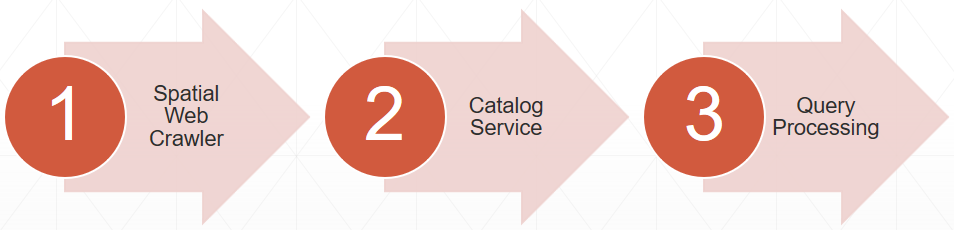
\includegraphics[width=\textwidth]{pix/flow}
  \caption{3 - staged pipeline approach}
\end{figure}
\newline
\item \textbf{Build Query orchestration service to perform real-time query with heterogeneous data sources and cost matrices associated with them.}
\par
One of the tasks of catalog service is to provide relevant information to the querying machine or person. The data that is stored by different repositories can be of heterogeneous form. Task of query orchestration is to find relevant information across all available data sources and perform the query using all relevant data. If the data is available from multiple data sources different type of ranking and cost matrices can be associated to provide most relevant information to the user. Query orchestration is also associated with ranking. While retrieving the data it should be presented to user in a ranked retrieval manner based on some metrics. Here we have discussed two techniques of ranked retrieval and indexing called Quad tree based indexing and ranking based on quality preferences.
\end{enumerate}

\section{Organization of thesis}
This thesis is mainly organized into six chapters. The first chapter gives introduction about the subject matter, it clears the motivation and advantages of the project. It defines the problem statement and states as well as explains the objectives of the project. The second chapter namely literature survey, provides already available data about the subject and proposed solution methods. This section first explains about the data for the model to be work with. It explains the web services and APIs build for spatial data. Then it explains about three part of the foundation platform, Spatial web crawler, Catalog service and query orchestration. Chapter 2 also discusses about the previous work done in the respective fields. 
\newline
\par 
Chapter 3, 4 and 5 are the core foundation blocks for Geo-service portal foundation platform. Chapter 3 is explains about the spatial web crawler. It explains the architecture and the algorithm used for the spatial web crawler. It also explains advantages of spatial web crawler. Chapter 4 contains information about spatial metadata discovery and publishing. It discusses objectives for the catalog service. It also give architecture and implementation details about catalog service for web and query processing. It also shows example results. It also extends the concept to cloud based paradigms.Chapter 5 gives a look into spatial query orchestration. It discusses about two broad strategies two index and rank spatial data.
\newline
\par
The final chapter concludes the morals of the thesis and creates a pathway for better optimizing and extending the proposed solution for the future work.
% \section{Development Platform}
\chapter{Literature Survey}
The literature for this project can be divided mainly into four parts. The spatial data and spatial web services on which the framework is developed. Crawling: How to find that data. Catalog Service: Once the data is found, how to store that data. How to make data easily accessible to others. And at the last Query orchestration: how to perform simple queries on the available data.

\section{Spatial Data \& Spatial Web Services}
\par
The term Geo comes from geography. Geography stores all the information of location and shape of the object in the spatial data. Spatial data stores the relationships between these data. It can also be easily mapped to a map. Spatial data is stored as raster data or vector data. Geo-server provides various kinds of functionality to this type of data. Spatial data is the data that can be mapped.Spatial data is collection of spatial object that has topology and co-ordinates. Spatial data gives geographical and shape related attributes of the data.Geographical information system is used to retrieve and operate on spatial data. Different operations can be add, visualize, annotate etc. A Geographical Information System provides various extended operation on spatial data. Different examples of such software that offers spatial services are ESRI, Microsoft SQL Server, ERDAS imagine etc.

\subsection{Classification of Spatial Data}
Open Geo-spatial Consortium(OGC) defines  Different types of object under the class geometry are as below. All the major Geo-spatial service providers and vendors provide this kind classification.The primitive four data types in spatial data are point, curve, surface and GeomCollection. Figure \ref{cosd} shows hierarchy in classification of spatial data.\\
\newline
\begin{figure}[h]
    \centering
    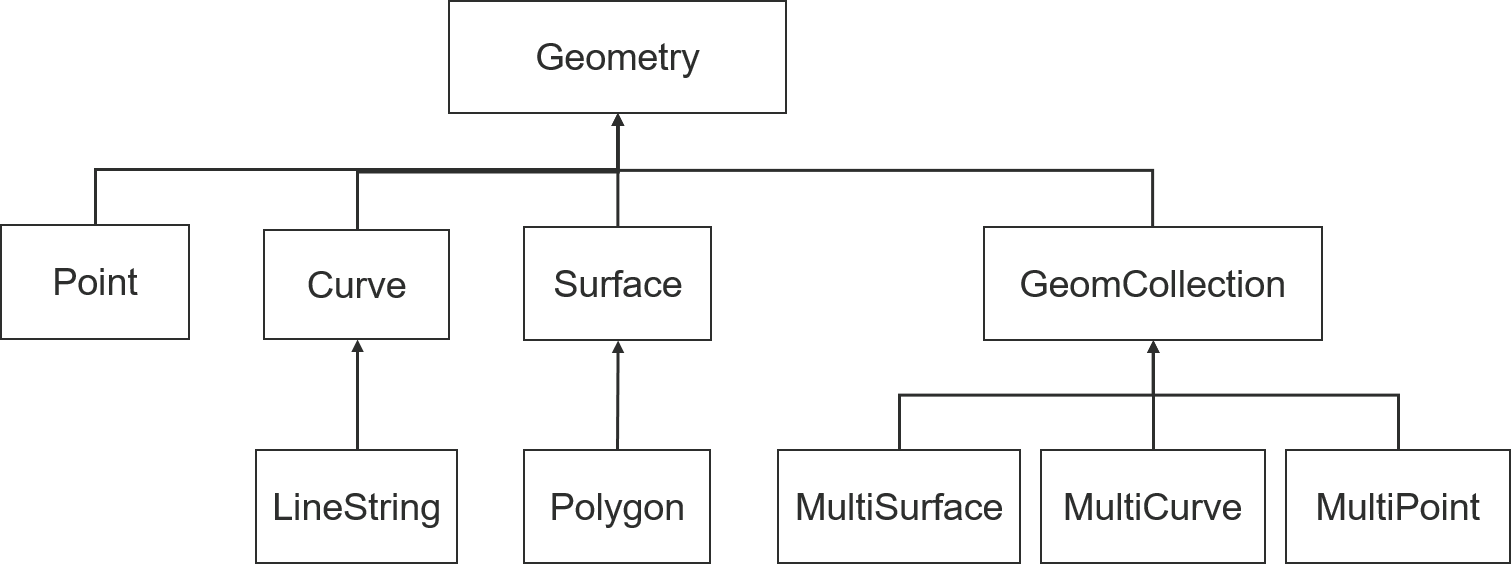
\includegraphics[width=\textwidth]{pix/p}
    \caption{Classification of spatial data}
    \label{cosd}
\end{figure}
\newline
\begin{itemize}
\item \textbf{Point}\\
Point in a map is denoted by (x, y) co-ordinates. When we see kharagpur city on a scale
of India it will be seen as a point. Point can be used to denote various objects like origin,
city, end point, top of the mountain etc. It denotes a single point consisting of longitude and latitude.\\

\item \textbf{Curve}\\
Curve is used to denote collection of points. This can be a straight line or curve. For
example, a road network can be represented with the help of line strings. Similarly, a
river can be denoted as a curve. Curve can be made with help of two distinct points.\\

\item \textbf{Surface}\\
A surface is representation of an area or a polygon. When kharagpur is seen in the scale
of west Bengal it is seen as surface or polygon. Polygon can be made using at least three non-linear points. Every polygon has a feature called boundary.\\

\item \textbf{GeomCollection}\\
Collection of basic building blocks defining a new type of geometry can be defined
with the help of GeomCollection. GeomCollection is made with combining two or more geometry types.\\

\end{itemize}


\subsection{OGC Web Services}
Open Geospatial Consortium (OGC) is the worldwide standardization body for geospatial standards. OGC provides a standardized way of accessing this geospatial data. OGC mainly provides three kinds of web services.\\
\begin{itemize}
\item \textbf{Web Map Service (WMS)}\\
Web Map service defines a way of accessing geospatial information across all geo servers in a
standard format as image. This image can be raster image or a vector image. Raster images are
of type jpg, png or bmp. Vector images contains svg format extension images. It also provides
a way to access metadata about the available information of the layers. This information can
contain type and no of layers. \\
Some of the well-defined operations in this layer are
GetCapabilities, GetMap and DescribeLayer. GetCapabilities operation returns capabilities of the server for example, what kind of services the server offers. This operation may be useful to check if a server is geo server or not by examining the kind of services it offers. GetMap service returns map images for the queried data. multiple such layer of images can be queried and then can be overlaid on top of each other. for example satellite view, terrain view, traffic view etc. Each of this layer gives additional information to the map. DescribeLayer operation describes what are the available layers and what is the metadata about the layers.\\
\item \textbf{Web Feature Service (WFS)}\\
WFS allows direct access to features contained in the map. WFS uses SOAP based interface. SOAP is used to minimize the overhead into the communication and verify cross platform stability.
For exchanging data between client and server WFS uses Geographical mark-up language(GML)
which is based on XML. Some well-defined operations in WFS are query or get feature, which
returns the feature stored on the server. We can add the feature in the repository by add feature.
We can delete feature by delete feature. Also we can update feature stored in the repository by
update feature. We can also lock certain feature to disallow modification of it while sharing via lock feature. Locked resources and features wont be accessible to change to other clients. Example of feature are the objects in the map like building or petrol pump.\\
\item \textbf{Web Coverage Service (WCS)}\\
WCS offers multi-dimensional coverage of the geo spatial data.It can provide originally retrieved data or provide processed data. It provides spatio-temporal
context to the given geographical data. For example, it can show the flow of the river changing
over the span of years. Thus we can say that WCS provides richer coverage of spatial data than
WFS or WMS. Coverage data is mainly used for scientific calculations.
\end{itemize}
\section{Spatial Web Crawler}
Spatial web crawler is a topical crawler which finds geospatial capable servers and services from the web. Sonal Patil\cite{l1} provides the base architectural guidelines for building spatial web crawler. Wenwen Li\cite{l2} says that if a server is offering geo-spatial capabilities then it can be either of the WMS, WFS or WCS server. The geo-servers must comply to OGC standards for geospatial data. This can be checked using GetCapabilities service request. We can check whether a given server offers WMS offerings or not can be checked using special suffix string added to the URL of a geo-server. More details are covered in the geo-spatial crawler part below. If the server is indeed a WMS server, It replies with and XML files containing all the data and operations it can offer. We call this as services.xml file. Once We know that the server is a geoserver many kinds of operations can be performed on it. WMS geoserver offer various operations such as GetMap, DescribeLayer, GetCapabilities etc. WMS capabilities file contains all these operations mentioned above. This is to check if a particular server is geoserver or not. If we want to crawl through the open web, then we must repeat this process. For this purpose standard operation of crawlers are performed. We maintain a buffer of frontiers which divides the boundaries of crawled web and open un-crawled web. Wenwen Li\cite{l2} also suggests to make a auto updating crawler to periodically check whether there is any addition or removal or geoserver from the existing available data. This geoserver(s) also add new data to them and remove obsolete data from the data store. Automatic updates allows this operations to be done periodically and maintain the overall consistency of the data.\\
\par
Marc Najork\cite{l3} suggests that the task of crawling the web for WMS servers can be done parallel. He suggests to use parallel FIFO queues to carry out the operation efficiently. To check whether the URL already exists or not in the crawled set, he suggests to use efficient data structures to check set membership such as HashSet. He also suggests to use priority in crawling based on various methods such as PageRank.\\
\par
Lopez-Pellicer\cite{l9} suggests that there might be already available geoservers and catalog services on the web. We must efficiently identify this catalog services to different type of OGC compliant services. So that different kind of queries can be forwarded to different geo servers or catalog services. Dirk Ahlers\cite{l4} suggests an architecture to crawl and parse available geoserver(s) and store the available data efficiently. They also suggests to index the data so there data can be retrieved efficiently. This methods is described as focused crawling.\\
\par
Li, W., et al.\cite{l5} suggest a method to semantically crawls the web. In his approach he maintains a hierarchy of geospatial objects to identify parent children relationship. For example, river is a type of water-body. This kind of type of relationships can be used to manage and index available data and geoservers efficiently. JIANG Jun\cite{l6} suggests similar methods for WFS servers.


\section{Catalog Service for Geo-Spatial Data}
Catalog service provides discovery and publishing of geospatial metadata information. Manoj Paul\cite{l14} provides a service oriented approach for discovery and retrieval of spatial data as web services. Nogueras et al.\cite{l15} discusses about design and storage mechanisms in a real world catalog service. 
\newline
\par In this section we will look at two types of available catalog services for geospatial data. Python catalog service for web(PyCSW)\cite{l7} offers a model architecture for implementing a OGC compliant web service catalog portal. In this model, series of module are used to invoke a hierarchy such that decomposition of the functions and use case is efficient and easy. In this architecture many of the modules can work in parallel. Important modules are crawler, WMS capabilities files, Database to store geospatial data and a server to provide interface to functions. All the functions are implemented and run via programs on a server. This wsgi server acts as a geospatial catalog which accumulates data from various other geospatial repositories and catalogs available on the open web. Using the PyCSW interface many types of applications can be invoked. PyCSW provides various APIs for OGC compliant operations. For example, using GetMap a user or application can get all the data from all the crawled repositories in a single place. We can know the information available for the layers and from where this information is available. The detailed implementation of this architecture is discussed in the later chapters.\\
\par
GeoServer\cite{l10} also offers such services but it also offers powerful management tools and admin console to function via graphical user interface. It provides services to work with various data formats such as shape files or GML format, it supports various database options for storage purpose and it is extensible to add more services. In our approach, we will mainly use GeoServer as our catalog service. However it should be noted that GeoServer is more resource intensive than PyCSW as it provides more services than the latter. It provides integration with various programming languages like Python, Java, Ruby and PHP.
\section{Query Orchestration}
Query Orchestration provides query operations on the spatial data from the database. Various operations are available as OGC standards to operate and query on the data. Query orchestration also deals with indexing and ranking. Here we have used Quad tree for indexing spatial data. Quad tree\cite{l13} is particularly standard data structure for indexing spatial data. Another interesting concept is ranking by quality preferences\cite{l11}. In this concept we take the cumulative property of spatial neighbourhood to calculate ranking for the spatial objects. Ranking data by quality preferences is a advanced method and requires extra information about quality of data.\\
\par
Once the catalog service is built it can directly act as a single point for querying multiple repositories. The catalog server in-fact acts as a mediator while getting the queried data from other repositories. Different type of example queries are listed below.

\begin{itemize}
\item \textbf{Service metadata information}\\
Describes what kind of OGC compliant web services are offered by the catalog server or geo-server.
\item \textbf{GetLayers}\\
An interface can be built to provide information about list of available layers.
\item \textbf{GetOperations}\\
List of available operations can be provided that gives the information about the list of operations that are offered by the geoserver or catalog service.
\item \textbf{GetBoundingBox}\\
We can get the information about the bounding box of the layers or map that covers the total area.
\item \textbf{GetMap}\\
The map of particular layer can be retrieved.
\item \textbf{DrawMap}\\
The map of particular layer/data can be retrieved and placed onto another map. This is useful to find area of interest in the particular map by superimposing the queried data to generic map.

\end{itemize}
\chapter{Spatial Web Crawler}
Our first step to building the platform Geo-Service portal is to gather the required spatial data. This can be done by finding the available data sources for geo-registries from the web via crawling or adding the sources manually. Spatial data is not indexed and available as compared to normal image or text data. The crawler module crawls the open web to find OGC compliant geoservers and stores their metadata information. It uses ontology or hierarchical mapping or spatial data to classify the crawled features. This features are permanently mapped into ontology to help in query processing.

% ---------------------------------------------------------------
\section{Objectives}
\begin{enumerate}
\item Build a spatial web crawler which crawlers through available geo-servers which offers WFS
based OGC compliant services.
\item Build a domain specific vocabulary(ontology) for this features which can be helpful to
compare found features with wanted features.
\item Perform semantic matching of found features from crawled web-pages with given
ontology for filtering the correct features and storing them in the permanent repository.
\item Perform an evaluation of the given spatial web crawler using metrics and test URL seed
sets.
\end{enumerate}

% ---------------------------------------------------------------

\section{Architecture of the Spatial Web Crawler}
Our crawler contains three modules for crawling spatial features through the world wide web.
Some of the definition needed for understanding the working of spatial web crawler are:\\

\begin{figure}[h]
  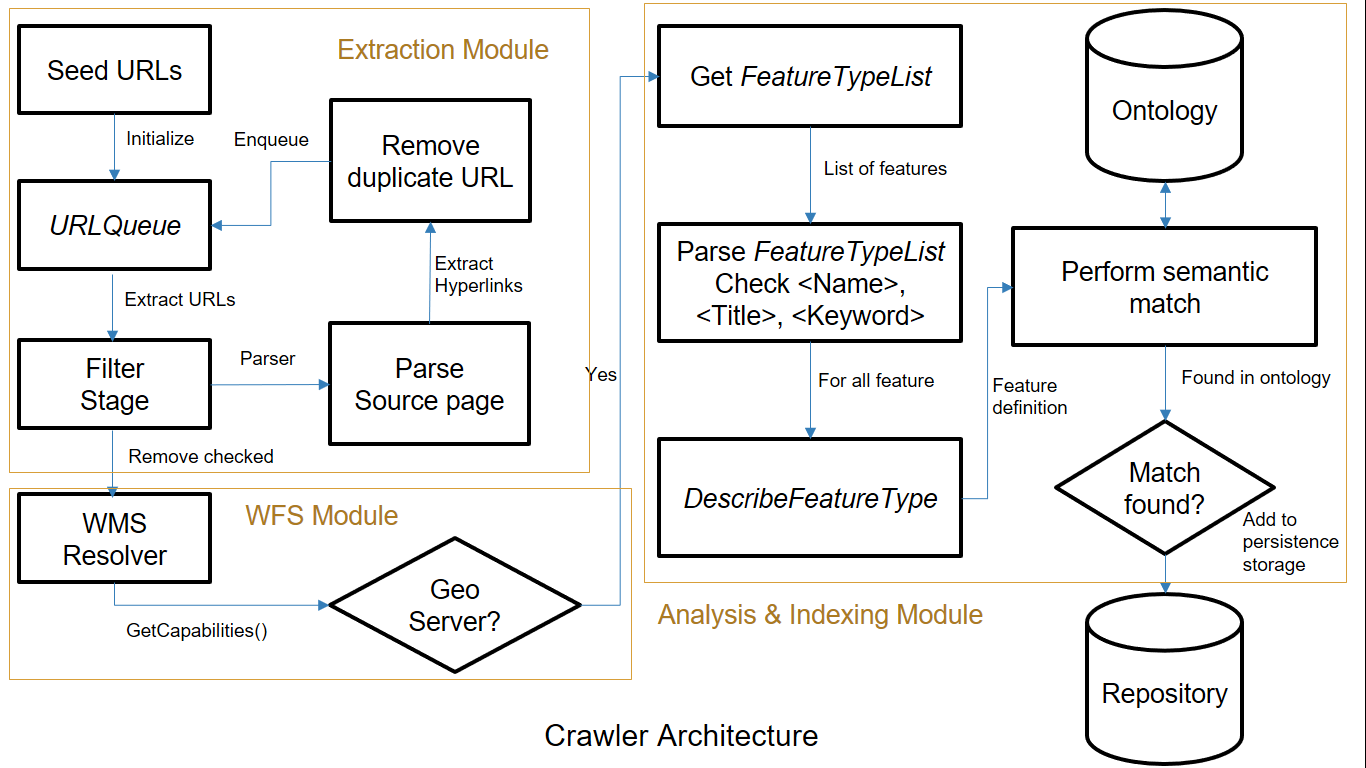
\includegraphics[width=\textwidth]{2}
  \caption{Spatial web crawler architecture}
\end{figure}


\begin{itemize}

\item  \textbf{Seed set}\\ A set of test URL(s) to initialize the queue for crawling the web. The crawler
starts with the URLs given in the seed URL set. Seed set URL(s) are processed and parsed to obtain other URL(s), which are added to the queue for later crawling.

\item \textbf{URLQueue}\\
A queue that contains set of URLs to be crawled. The crawler module takes URLs one after the another from this queue. It contains list of all the valid URL(s) to be crawled. It contains seed set initially. URL(s) are taken one by one by the crawler module for processing and deleted from the URLQueue. Similarly, newly found URL(s) are added to the queue.

\item \textbf{Frontiers}\\ 
A set of URLs from the URLQueue that are currently being crawled. This are
called frontiers because they reside between the known web and the unknown web. This are active URL(s) currently participating in the process of crawling. Frontiers are checked by the WMS resolver module for their geo-capabilities and parsed by extraction module to get new set of URL(s) to add in URLQueue.

\item \textbf{WMS resolver}\\
WMS resolver is a module that checks that if a server is WMS server
or not given the URL from the URLQueue. It uses special request URL to check whether the server replies to the URL in an OGC compliant manner. 

\item \textbf{Parser}\\
Parser is a module that downloads the webpage from the given URL and parse
the HTML webpage looking for pre-specified tags and names. After parsing it gets a
set of tags and its contents. In our implementation we parse the webpage and look for
the anchor tags within it and store all the hyperlinks from the crawled webpage. This links are then stored in the URLQueue for further processing.

\item \textbf{Ontology}\\ 
Ontology is a semantic dictionary containing all the features its type and relationship
hierarchy between features. This is used while mapping features to it's corresponding super-type and while query processing that contains more than one feature type. For example, getting overlap or intersection between two feature types.

\end{itemize}
Spatial Web Crawler is designed to contain three modules. This modules are namely Extraction module, WFS module and Analysis \& Extraction module. They are designed in a manner that they can work independently, which will come useful while implementing this as a extension in cloud based environments. :

\begin{itemize}

\item \textbf{Extraction module}\\
Our algorithm starts with a set of seed URLs contained in the seed set. We initialize the
URLQueue with these seed URLs. Initialization is done manually. It is required to choose these seed set URL(s) carefully, to get better results in crawling. Ideally, seed URLs should be good authorities, they should point to large number of good geoserver(s). Depending on the seed set, the crawler module may find more and less no of good spatial repositories in less or more amount of time. The crawler takes URL from the URLQueue and feeds it into filter stage. The filter stage takes the URL and checks
whether the given URL is already crawled or not. After filtering such URLs, they are sent to
the parser. The parser downloads the web-page from the given URL and parses it for finding
hyperlinks contained in it. These hyperlinks again go to filter stage for finding whether the
given URLs are already crawled or not. After filtering these URLs are added to the end of
URLQueue. The filtered URLs are also passed to the WFS module.\\

\item \textbf{WFS module}\\
Once the URL is fed into WFS module for the examination, WFS module sends a GetCapabilities() request to that server.
We do this by appending the request to the URL.
\begin{center}
$?
  service=wfs\&
  version=1.1.0\&
  request=GetCapabilities$
\end{center}
The server replies for this request. If the reply contains WFS\_Capabilities tag, then it offers
WFS service. We parse the received response for finding the WFS\_\\Capabilities tag. The server replies in XML format usually called capabilities.xml file, this files contains all metadata information about the feature services offered by the WFS server like number of layers, type of operations supported, feature description, etc. If the given
server is WFS server then the given URL is passed to analysis and indexing module.\\
\item \textbf{Analysis and Extraction module}\\
In this stage server response is parsed for the tag FeatureTypeList. FeatureTypeList
contains list of features. This features are stored under the tag FeatureType. FeatureType
tag contains set of keyword, title, name tags. Each of this tags are checked to see if it
contains any word from the ontology. For each of such tag found, DescribeFeatureType request
is appended to the URL.

\begin{center}
$“?service=WFS\&version=1.1.0\&request=DescribeFeatureType\&typename="+keyword$
\end{center}

Here the keyword is the name of the feature. Each of this retrieved feature is checked again
the ontology, if similar feature is found in the ontology then it is added to permanent storage in
the repository. Matching is done semantically via ontology. 
\end{itemize}

\section{Algorithm}
The \textit{Extraction algorithm} is used to crawl and parse webpages. It parses the available URL by downloading the webpage and extracts the anchor tags and corresponding URL(s) associated with it. It passes these URL(s) to \textit{WMS Resolver} module.
\newline
\begin{algorithm}[H]
	\caption{\em Extraction Algorithm }
	\textbf{Input:} set of URLs to start crawling \\
	\textbf{Output:} set of WMS capable URLs 
	%\begin{minipage}{\linewidth}
	\begin{algorithmic}[1]	 
	
	\algnewcommand{\Initialize}[1]{%
        \State \textbf{Initialize:}
        \Statex \hspace*{\algorithmicindent}\parbox[t]{.8\linewidth}{\raggedright #1}
        \newline
    } 
    
    \Initialize{
        \FOR{ URL in Input}
            \State $URLQueue.insert(URL)$
        \ENDFOR
    }
        
    \FOR{URL in URLQueue} 
        \IF{! filter(URL)}
            \STATE $preUrlSet \gets parser(URL)$
            \STATE $urlSet \gets filterDuplicate(preUrlSet)$
            \State $URLQueue.insert(urlSet)$
        \ENDIF
        \State $WMSresolver(URL)$
    \ENDFOR 
	\end{algorithmic}
\end{algorithm}
\par \textit{WMS Resolver} module checks if the URL provided by the \textit{Extraction algorithm} corresponds to a spatial repository or not. It does this via making standard OGC web service calls to the given URL. If The URL is found to be a spatial repository it is then forwarded to the Analysis and Indexing module. No actions are taken otherwise.
\newline
\begin{algorithm}[H]
    \caption{\em WMS Resolver Algorithm }
    \textbf{Input:} URL to check for OGC compliant services \\
	\textbf{Output:} WMS capabilities
	
	\begin{algorithmic}[1]
    \State $Response \gets GetCapabilities(URL)$
    \IF{$Response$ contains $WMS\_Capabilities$}
        \State $Analyze(URL)$
    \ENDIF
    \end{algorithmic}
    % \addtocounter{algorithm}{-1}
\end{algorithm}
\par The aim of \textit{Analysis \& Indexing} algorithm is to retrieve and store spatial features from the given URL. The algorithm first makes a request to get all \textit{FeatureTypes} from the spatial repository. For each \textit{FeatureType} it checks if the type matches semantically with the ontology. Matched features are stored into the repository.
\newline
\begin{algorithm}[H]
    \caption{\em Analysis \& Indexing Algorithm }
    \textbf{Input:} WFS capable URL \\
	\textbf{Output:} WFS records
	
	\begin{algorithmic}[1]
	    \State $FeatureTypeList \gets GetFeatureTypeList$
	    \FOR{ $feature in FeatureTypeList$}
	        \State $name \gets feature.name$
	        \State $description \gets DescribeFeatureTypeList(feature)$
	        
	        \IF{ $(name,description)$ matches in $ontology$}
	            \State Store record in repository
	        \ENDIF
	        
	    \ENDFOR
	\end{algorithmic}
\end{algorithm}

\section{Example Scenario \& Results}
Suppose we search for a example query after building the system. Let this query be \textit{river and snow}. Now if we search this on normal search engines like Google, it will show us results containing either river or snow. But as we have information about spatial context in this crawler. Repositories have stored the information about which features are in near proximity to each other.
\newline
\par
Other than this, we have a object ontology. Which is a hierarchical graph based on the spatial features. This graph contains generalized and specialized features. For example it suggests that river comes under the type stream which intern comes under the geometry type waterbody. This type of hierarchical classification helps us to understand the geospatial data and their features and relationships correctly. Our query is river and snow. The crawler searches the repository for finding both features river and snow or their similar representation by doing a semantic matching over ontology. Once found it can see which is the geo server which offers both of the geo services and feature types. Based on its finding from the repository we conclude our results and send the reply back to the user.
\newline
\begin{figure}[h]
    \centering
    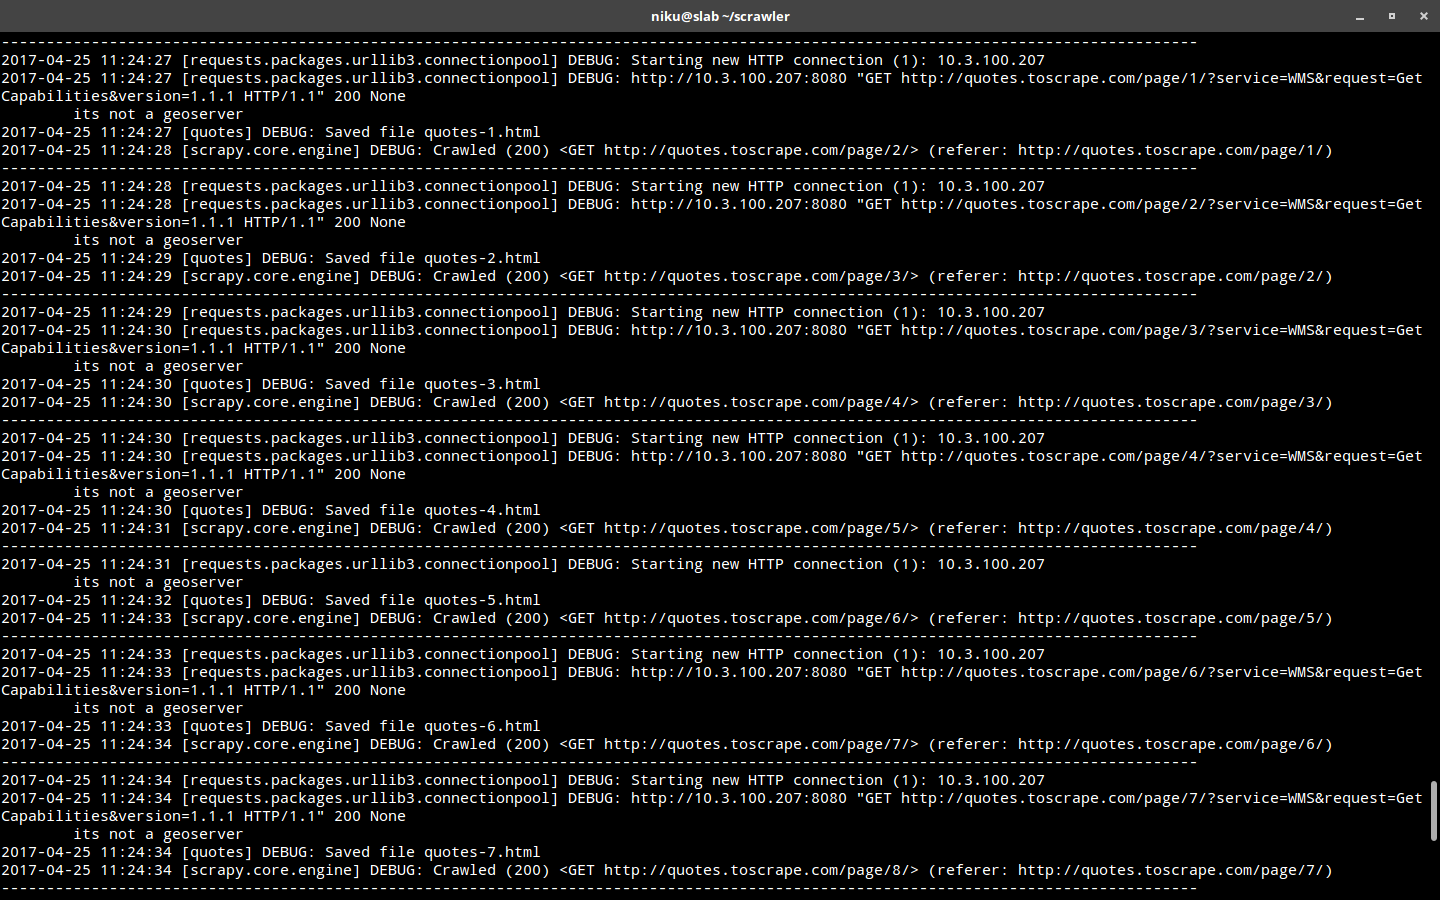
\includegraphics[width=\textwidth]{pix/p14}
    \caption{Spatial Web Crawler Implementation}
    \label{3.3}
\end{figure}
\newline
\par
Spatial web crawler is implemented with the help of Scrapy(\textit{https://scrapy.org/}) framework. It is a very powerful tool to crawl and scrap web pages. For each crawled URL, we pass it on the \textit{WMS\_Resolver} module to check if it is a spatial repository or not. Spatial GeoServer or catalog servers replies to GetCapabilities request with an XML file, part of which can be seen in the figure \ref{3.2}.
\newline
%%%%%%%%%%%%%% figure %%%%%%%%%%%%%%%%%%%%%
\begin{figure}[h]
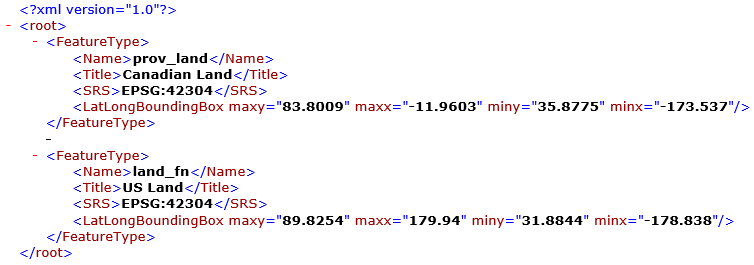
\includegraphics[width=\textwidth]{1}
\begin{center}
\caption{XML response from the geo server}
\label{3.2}
\end{center}  
\end{figure}
%%%%%%%%%%%%% figure end %%%%%%%%%%%%%%%%%%
\par
If the URL is not geo spatially capable, It is skipped as shown in the figure \ref{3.3}. For each URL the script prints if the URL is a GeoServer or not. If the URL is found to be a GeoServer, the response related to it is stored as XML and is further parsed and processed by catalog server.

\section{Advantages of Spatial Web Crawler}

\begin{itemize}
\item  Allows search in web pages that are not generally searchable from the normal search
engines. This is because of the spatial context awareness of the spatial web crawler.
\item It provides more up-to-date results from the results. Spatial crawler is more sensitive to
changes of spatial data on the web and automatically crawls through the changed
features with the help of automatic update module.
\item Provides improved accuracy in the search of spatial features and operations.
\item Provides extra features such as bounding box of spatially crawled data and other spatial
features. This bounding box can then be used for visualizing the crawled data.
\item Spatial data mining and analysis kind of tasks can be performed. So that we can infer and predict new results and patterns.
\end{itemize}
\chapter{Spatial Metadata Discovery \& Publishing}

Once the geo-servers are crawled from the open web, we need to organize this data into a well organized manner so that it can be retrieved efficiently. The operation and query we perform on this data must be performed in a efficient manner. The aim of Spatial metadata catalog server is to make crawled spatial metadata available for public.

\section{Objectives}

\begin{enumerate}
    \item Parse the crawled metadata and store it into a permanent database in a structured manner.
    \item Publish metadata repository in OGC compliant manner to make it available as a service.
\end{enumerate}

\section{Architecture of Catalog Service}

 There are various data repositories available on the web. However this repositories are not indexed. Spatial web crawler crawls through open web and stores corresponding metadata information about available data into the xml files. Crawler uses \textit{GetCapabilities()} OGC request to find if a given server is geoserver or not, if the given URL is indeed a geo-server then crawler module requests to retrieve \textit{capabilities.xml} file from the server and stores it into warehouse. XML files contains the services information provided by the geo-servers found on the web. They are usually called services.xml.
 \begin{figure}[H]
 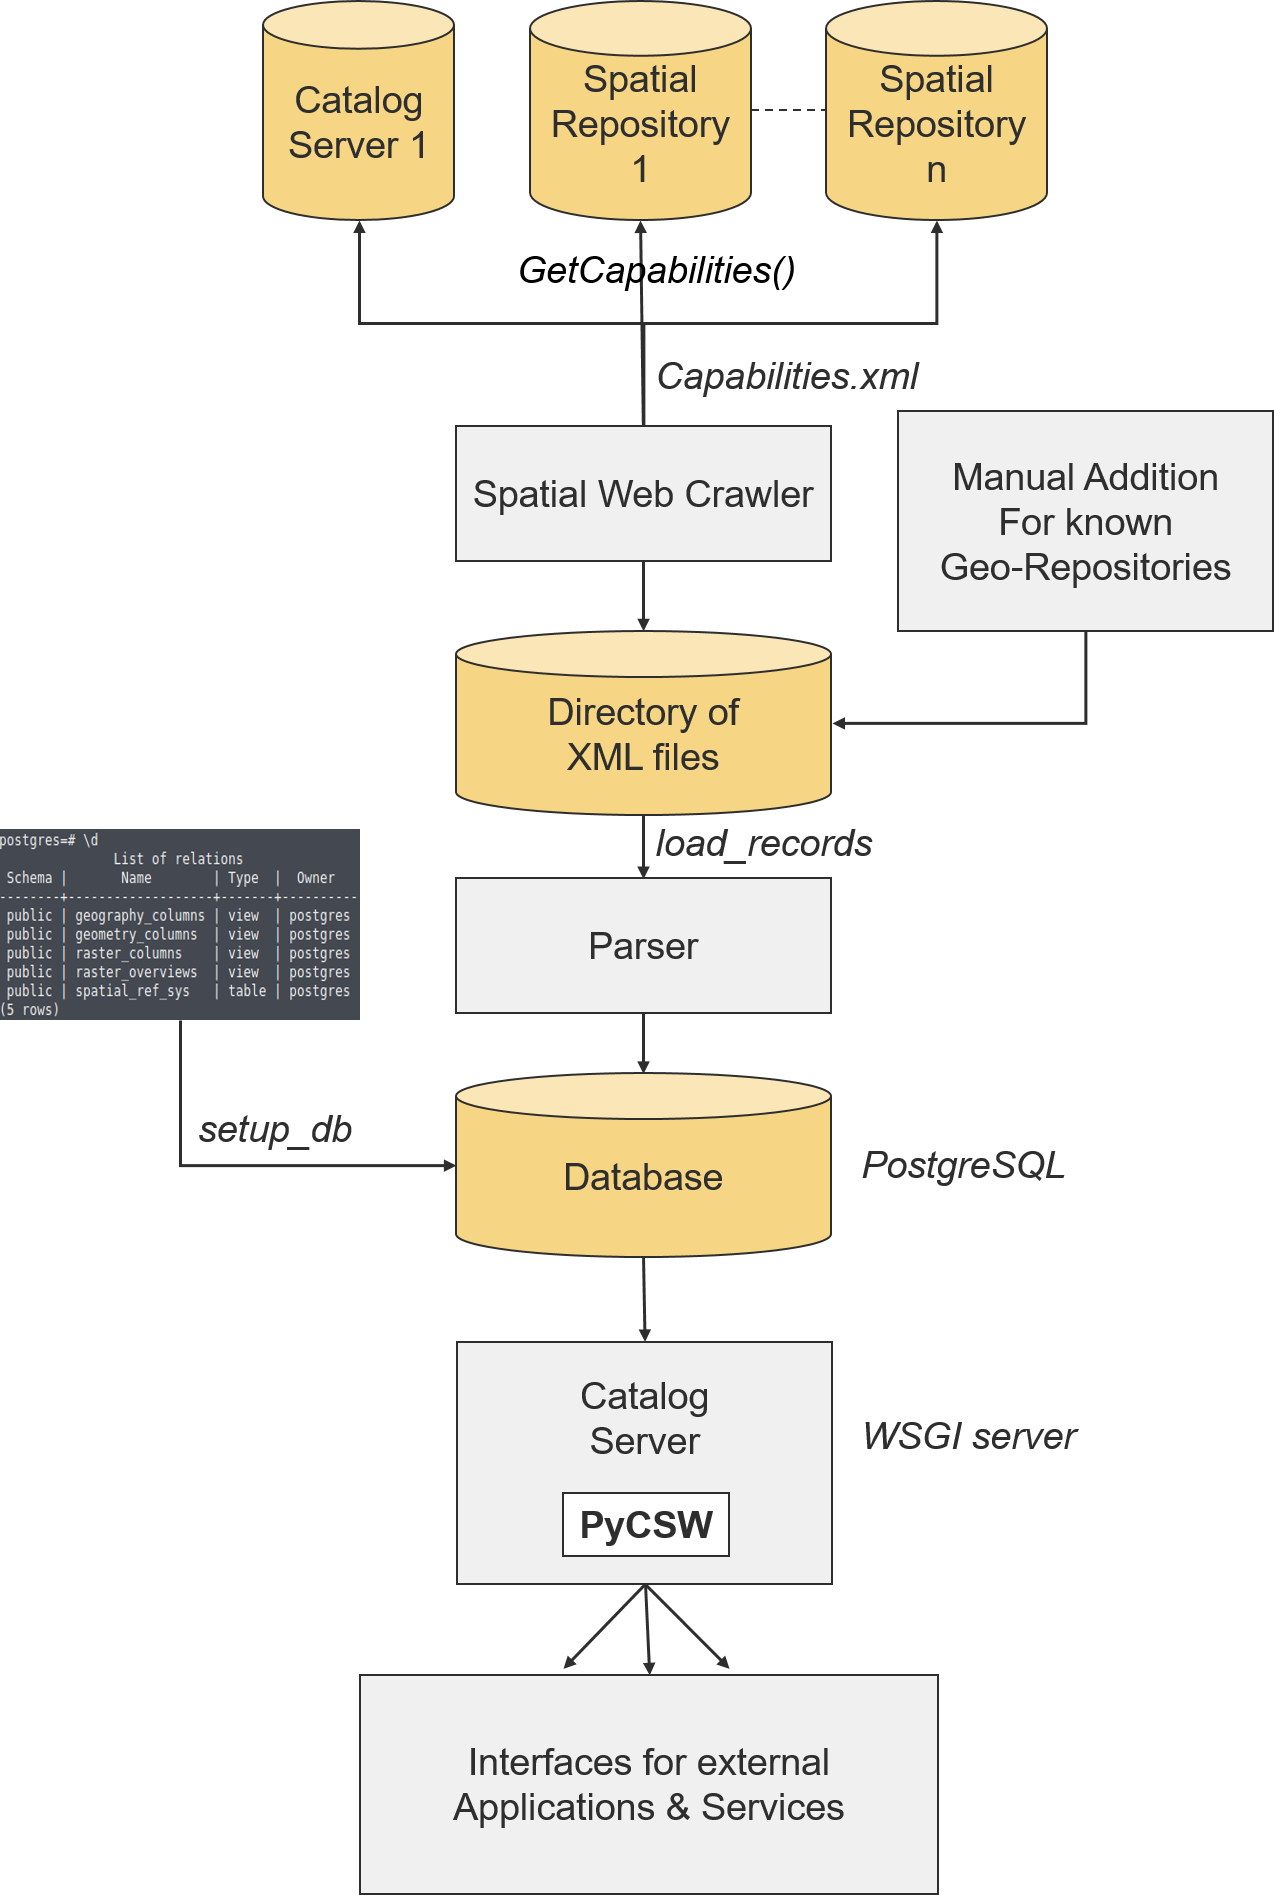
\includegraphics[width=\textwidth]{pix/Picture3}
 \caption{Architecture of Catalog Server}
 \end{figure}
 This information contains available operations, available layers and other useful information. This xml files are gathered in a folder containing xml files.\\



% \begin{figure}[h]
%   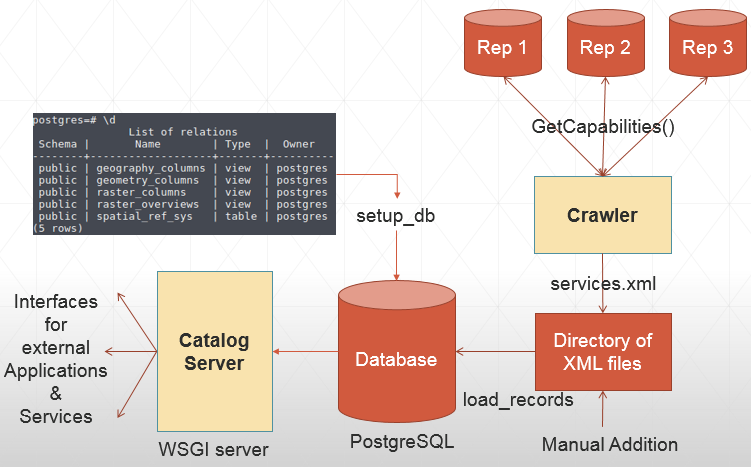
\includegraphics[width=\textwidth]{7}
%   \caption{Architecture of Catalog Service}
% \end{figure}

\par No of spatial repositories in the web is significantly lower than other type of services and servers. It can happen that it might take a significant amount of time to gather practically good number of geo-servers. For this reason, this files can be added by the spatial web crawler or it can be added manually.
\newline
\par This xml files are then loaded into the database for faster and efficient retrieval operation. For database we can use either of MySQL, PostgreSQL or SQLite. But MySQL and SQLite does not offer inherent data structures and operations support for spatial data. SQLite is also meant for light weight databases, whereas here the no of request-reply and data transfer can be very high. For these reasons it is better to choose PostgreSQL database system to store data for the catalog service. PostgreSQL offers high scalability and offers inherent support of spatial data types and operations.\newline
\par Catalog Service is hosted on \textit{Web server gateway interface (WSGI)} server. We can also use other deployment servers like Apache. Main reason for choice of server as WSGI is that, WSGI integrates well with python. It is build on python. It is useful for request-reply type ordinary web interfaces and it is efficient for file transferring on other protocols. A python program admin.py is hosted on WSGI server, which takes the metadata information from the database and replies in response to GetCapabilities() request. When working on a particular request for a repository like GetMap(), the catalog service acts as a mediator between client and the repository on which the data is hosted. It converts the request taken by WSGI server converts it into standard OGC compliant WMS or WFS call, and accesses data from original repository from where data is hosted.


\section{Implementation}
There are two types of implementation done to implement catalog service module. First implementation covers $PyCSW$ python catalog service for web and second implementation makes use of $GeoServer$ open source tool for sharing spatial data. Difference between two type of tools is while PyCSW offer great functionalities and most of the OGC compliant services, GeoServer also offers more data type support to load repository from and a management console for admin to maintain Geo-registry. We will take a look at both type of solutions here.

\subsection{Crawler Module}

In first stage implementation, we first crawl through open web using the spatial web crawler discussed in the above chapter. The crawler checks if the given server provides geospatial services or not. If the server is a geospatial repository then it collects all the metadata information about the repository and stores it in a form of a xml files. Standard OGC compliant service calls are used for collecting metadata information about found registry. Here in the figure we can see there are three repositories which have been crawled by the crawler. The information about these repositories are stored in a xml files called services.xml. The no of geoservers and registries are very less in the open web compared to other kind of services, for this reason it might take a long time to crawl and find significant amount of registry services for our catalog service. To handle this problem, manual addition option is used. We can manually add popular geoservers and registry services to the services.xml files. We know that geoservers reply in xml response when called for a $GetCapabilities$ request. We can use this property and manually add popular geo-registries beforehand to the set of xml files. So in the summary, the first stage crawls the web and stores corresponding set of services files into one place.
\newline
\par For this, python based crawler module program is used. It takes a set of seed URLs, checks if the URL can built object of OGC compliant WMS or WFS object. If it can build OGC WMS object then, crawler requests for capabilities file, and stores it in set of xml files.


\subsection{Database Setup}
In second step, These set of xml files are used to populate database. Here various type of databases can be used. I have tried databases like MySQL, SQLite and PostgreSQL. In our approach I have used PostgreSQL because it offers geospatial properties and services inherently. Other databases do not offer inbuilt services for spatial data. PostgreSQL database offers PostGIS extension, which are a set of libraries to extend PostgreSQL database into spatial database. For adding PostGIS to PostgreSQL, go to PostgreSQL shell psql and create a extension, PostGIS. 

\begin{center}
\textit{CREATE EXTENSION POSTGIS;}
\end{center}

\par Once this is done, import all of the services,xml files into the database. Create structured tables and schema for maintaining spatial data. For this purpose \textit{setup\_db} command is used from catalog service module.

\begin{figure}[h]
\centering
  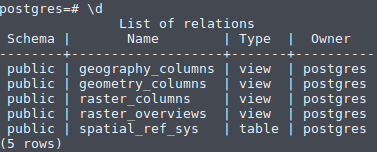
\includegraphics[width=0.8\textwidth]{8}
  \caption{List of relations}
\end{figure}

\par Here four tables are built to store and index spatial data efficiently. Those are, $geometry\_columns, records$ , $spatial\_ref\_sys$ and $spatial\_ref\_sys\_srid\_seq$. This tables are then used by the catalog server to publish and query available data. When a external entity queries catalog server for Get Capabilities request, the catalog server replies with the services file which contains all the information about all the geo-servers it has crawled till now. Thus it contains all the layer information and data crawled from the Internet. This makes it a single point of resource access. Data from xml files is parsed and stored into respective relations. For this \textit{load\_records} command is used from admin.py module within PyCSW. These tables are used to store parsed spatial features from the spatial repositories.

\subsection{Catalog Service}
Catalog service takes all available data from the database and creates a metadata capabilities file. It acts as a mediator between repositories which actually contains the data and the client. When a client requests for a query or a metadata service, catalog service checks if the database contains the information. If metadata information is requested, it replied directly to the client with the necessary files or response.\\
\begin{figure}[h]
\centering
  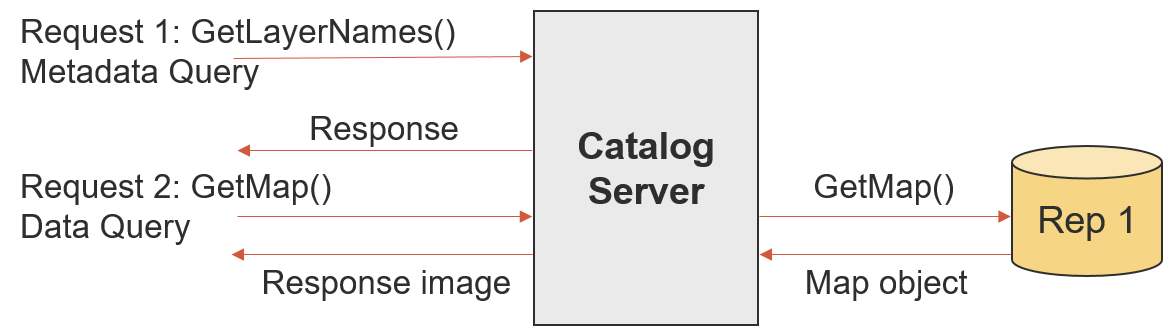
\includegraphics[width=\textwidth]{pix/Picture5}
  \caption{Catalog Service as a mediator}
\end{figure}
\par In case of query requiring actual data instead of the metadata, the catalog service resolves the source from which the data is available and brings the data back to the requester client. In this case, the catalog service acts as a mediator between client and the data source, acting just as a catalog. Here the catalog service is implemented via GeoServer. GeoServer takes the crawled layers from web map service and loads it into catalog.

\subsection{Query Processing}
When a query or request for the data is processed by the catalog service, it acts as a mediator between client and the repository from which the data is intended. It creates a object of the required service and requests for the object on behalf of the client. Client authorizes to the catalog service and catalog service authorizes itself to the data repositories for the transfer of data. Catalog service takes the object response from the repository and send it in response to client in client specified format. For metadata queries the catalog service retrieves data from database via object relational mappings in programming paradigms, this helps when having a multiple references to same object or feature. This method is used for retrieval of the features. How the featured are retrieved and presented are discussed further in the chapter 5.


%%%%%%%%%%%%%%%%%%%%%%%%%
\section{Extending catalog service with cloud characteristics}
A key logical step to scale catalog service for the larger audience is to make a cloud based implementation. Cloud based implementation has characteristics like scaling horizontally, high availability and dynamic dispatch of machines. To achieve the effects of scalability and high availability, we can make use of $load\_balancer$, $load\_balancer$ is a machine that acts as a middleware between client request and actual catalog servers. It forwards the request to one of the servers based on some qualitative features.
\newline
\begin{figure}[h]
    \centering
    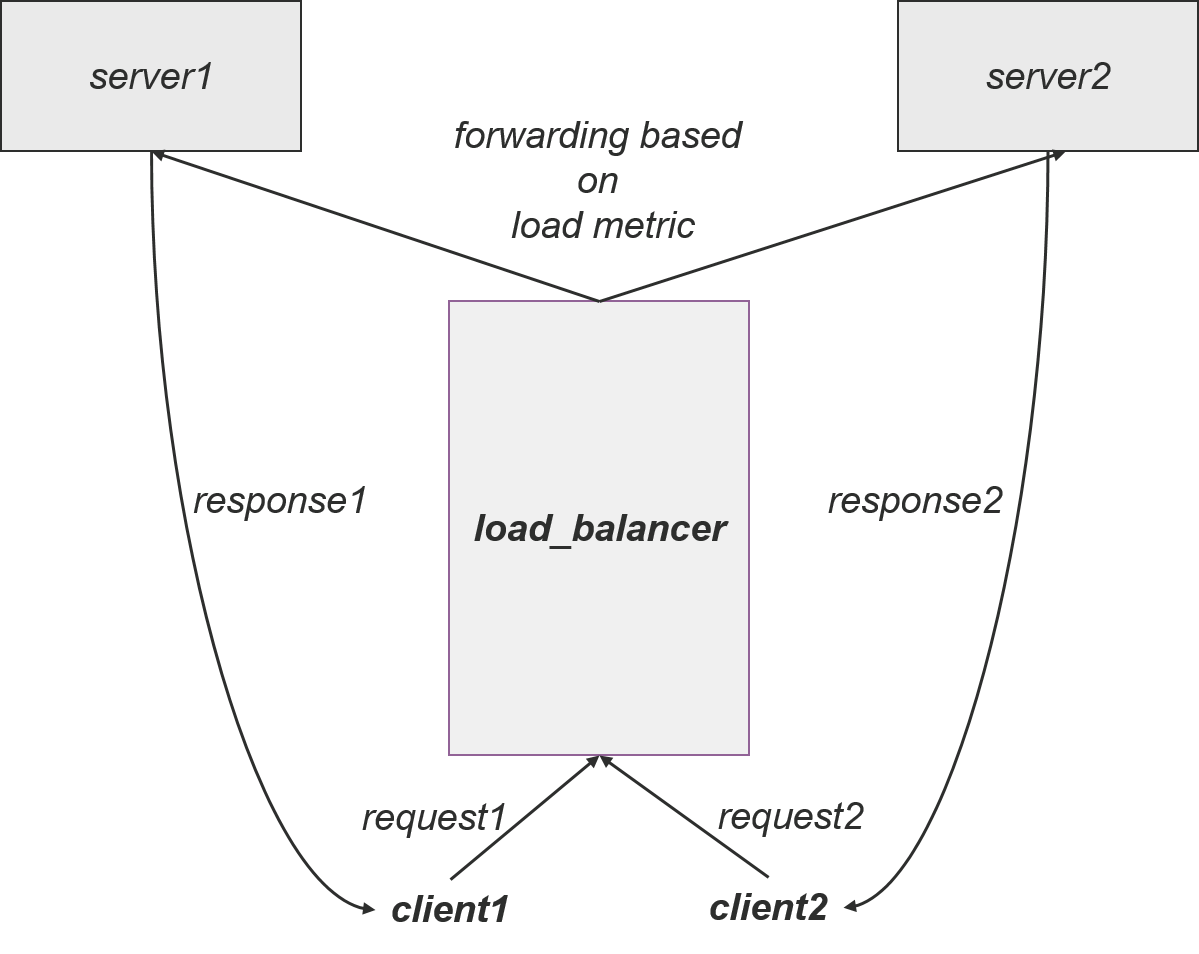
\includegraphics[width=0.7\textwidth]{pix/Picture7}
    \caption{load balancer implementation}
    \label{p7}
\end{figure}


\par In our approach, we have started by building a $load\_balancer$ which balances the requests between multiple available given geoservers. These geoservers are cloned to provide similar functionality but high availability. $load\_balancer$ detects which server has low number of requests compared to others and forwards the request to particular server. Actual servers are transparent to the end users. Interface between client and the geoservers is the $load\_balancer$. It acts as a gateway for connecting with the geoservers. In our test implementation, we have created two instances of geoservers and run similar repositories on each of them. The client connects to the $load\_balancer$ which acts as a gateway for the actual geoservers. It gets the reply back from the actual servers and sends it to requesting clients. $load\_balancer$ can also restrict or allow certain users grant on certain function and not all of them, thus here $load\_balancer$ also acts as a control panel and authorization entity for the access control.
\newline
\begin{figure}[h]
    \centering
    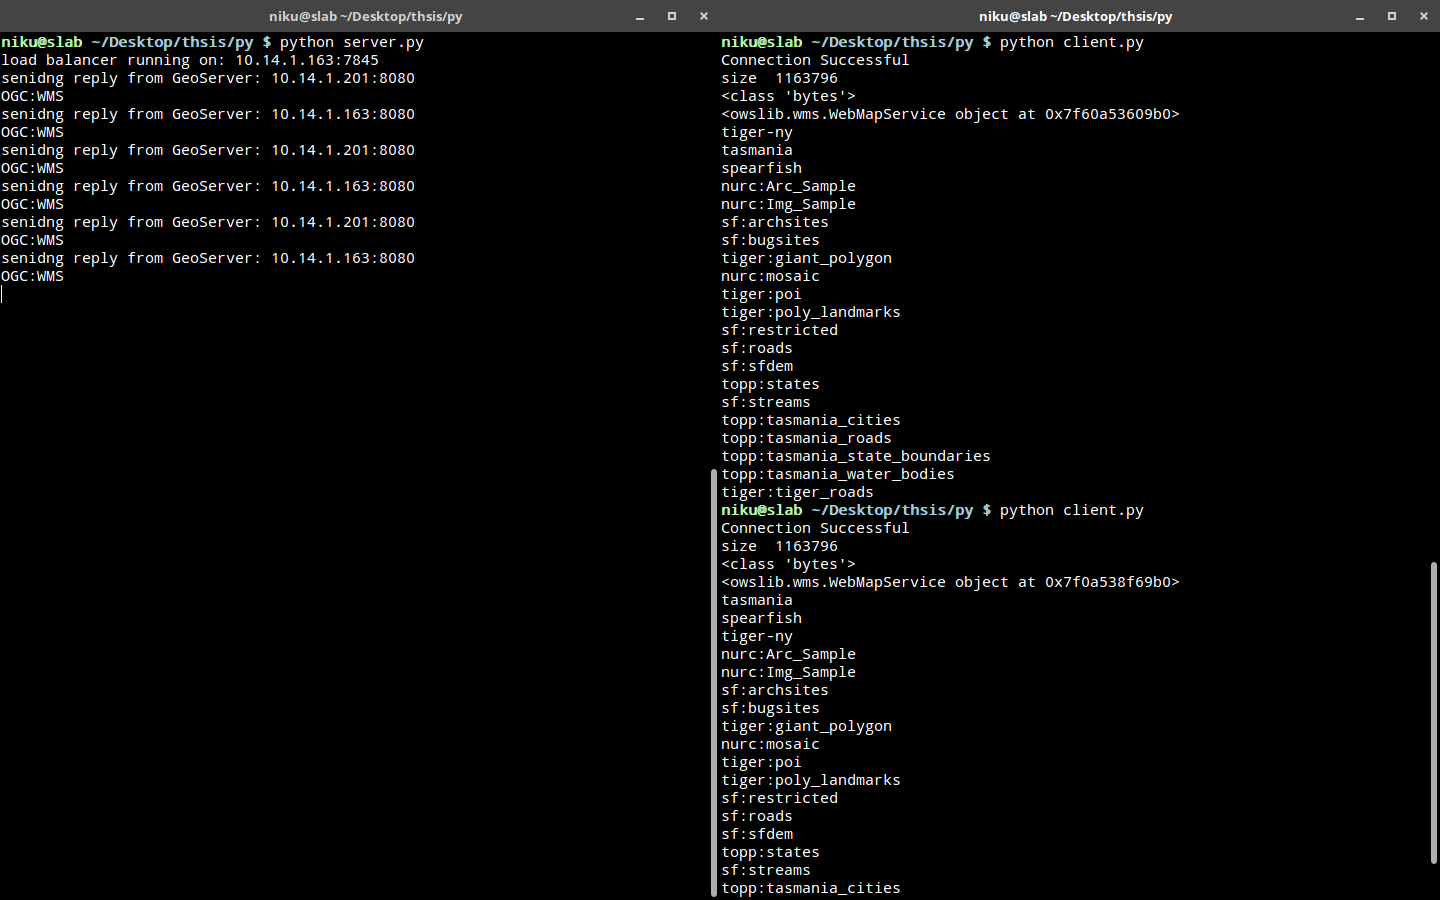
\includegraphics[width=\textwidth]{pix/p13}
    \caption{load balancer preliminary results}
    \label{p13}
\end{figure}
%%%%%%%%%%%%%%%%%%%%%%%%%
\section{Results}
Here are some results from the projects that explains and elaborates what kind of information can be get from catalog service. We have connected to GeoServer instance that is locally hosted. Note that many more richer services can be added to the platform to extend it's functionality.

\begin{figure}[h]
    \centering
    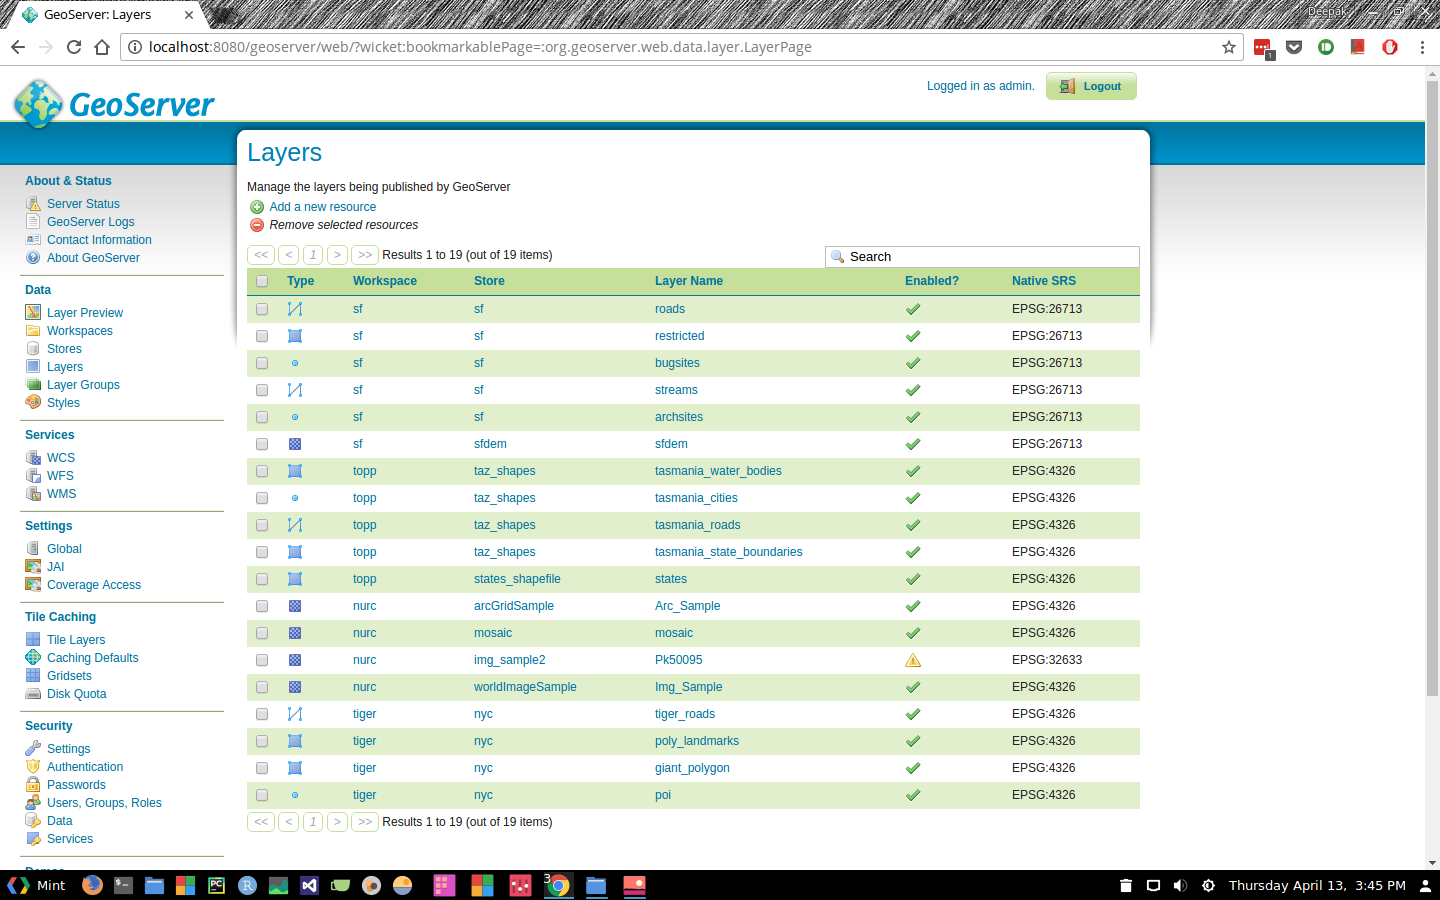
\includegraphics[width=\textwidth]{pix/p8}
    \caption{GeoServer Implementation}
\end{figure}

\begin{itemize}

\item Information about service metadata : OGC:WMS\\
This shows that registry is capable of providing OGC compliant web map service type of service to the user.\\

\item Title : GeoServer Web Map Service\\
Title gives information about title of the server hosting web map service.

\item List of available layers
\begin{enumerate}
\item kgp:POPULATION 
\item kgp:bnk\_block\_boundary 
\item kgp:bnk\_block\_hq 
\item kgp:bnk\_district\_boundary 
\item kgp:bnk\_drainage 
\item kgp:bnk\_grampanchayat\_boundary 
\item kgp:bnk\_mouza\_boundary 
\item kgp:bnk\_road
\item tasmania
\item spearfish
\item tiger\-ny
\item nurc:Arc\_Sample
\item nurc:Img\_Sample
\item sf:archsites
\item sf:bugsites
\item tiger:giant\_polygon
\item nurc:mosaic
\item tiger:poi
\item tiger:poly\_landmarks
\item sf:restricted
\item sf:roads
\item sf:sfdem
\item topp:states
\item sf:streams
\item topp:tasmania\_cities
\item topp:tasmania\_roads
\item topp:tasmania\_state\_boundaries
\item topp:tasmania\_water\_bodies
\item tiger:tiger\_roads
\end{enumerate}

This shows the list of available data in the form of layers. Each layer represents data of a geographic location from a view point. Multiple layers can be overlapped on each other to better understand the data. Each layer contains multiple features in itself. 

\item Available operations (WMS)
\begin{enumerate}
\item GetCapabilities 
\item GetMap 
\item GetFeatureInfo 
\item DescribeLayer 
\item GetLegendGraphic 
\item GetStyles 
\end{enumerate}

Gives details about the operations that can be performed by the geoserver. For example, DescribeLayer provides information about a particular layer. GetMap returns a map of layer in multiple available formats. 

\item GetMap\\
\begin{figure}[H]
	\centering
  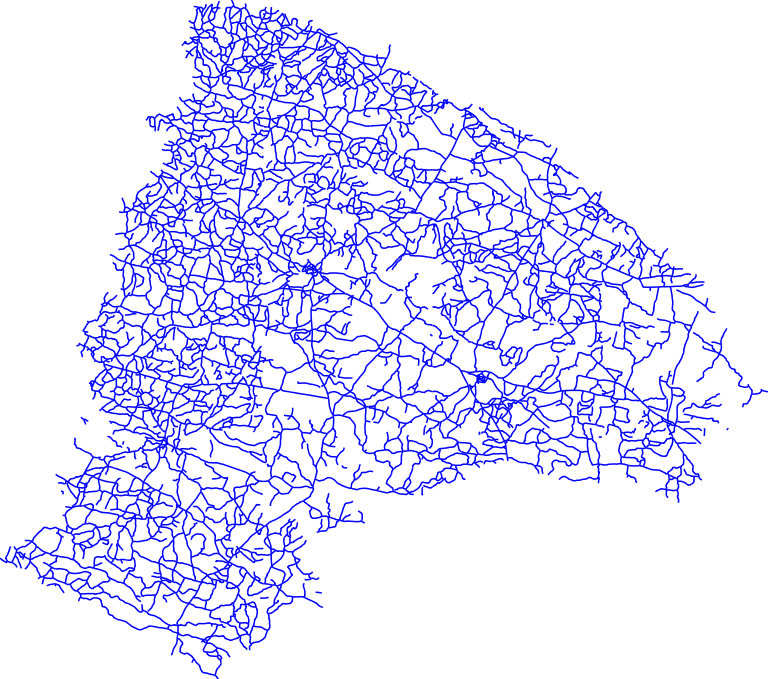
\includegraphics[width=0.7\textwidth]{bnk}
	\caption{Map of KGP BNK ROAD}
\end{figure}
Returns a map of particular layer. Can be superimposed to another map for better visualization. GetMap supports multiple options like name of layer(s), styles, transparency, bounding box, size and format like jpeg, png or pdf. 
\item DrawMap\\
DrawMap overlays different map images on top of each other to better visualize and analyze the effect of desired operation. For example, it can be used to find area affected by flood, or to find division of regions based on religion.\\
\begin{figure}[H]
	\centering
  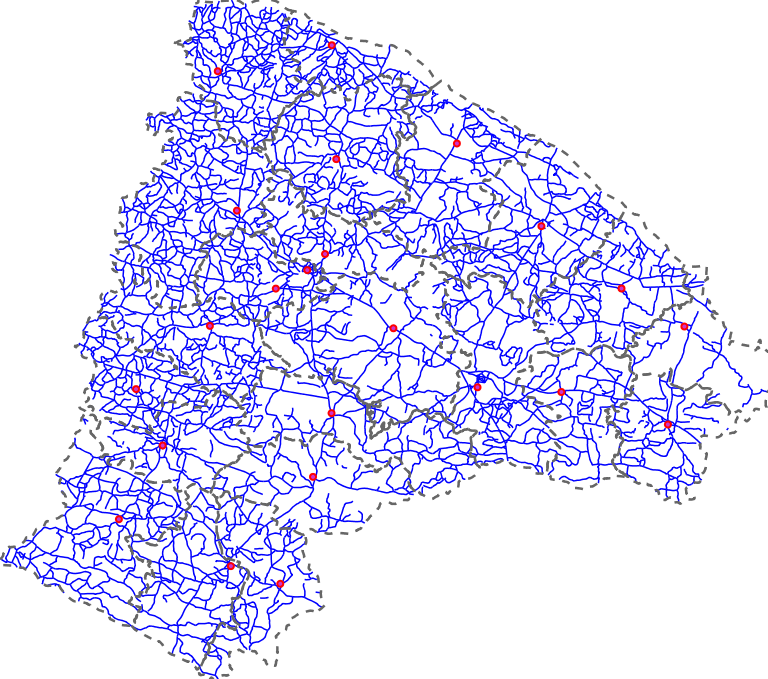
\includegraphics[width=0.7\textwidth]{9}
	\caption{Overlay of KGP BNK ROAD, Block HQ \& Boundary Layers}
\end{figure}
User can specify options to get the result image in desired format.\\
Options:\\
Layers = \{ kgp:bnk\_road, kgp:bnk\_block\_hq, kgp:bnk\_block\_boundary \}\\
Width = 768\\
Height = 679\\
Format = image/png

\item Information about specific layer: 
\begin{itemize}
\item Title --- POPULATION 
\item Name --- kgp:POPULATION 
\item Is Queryable --- 1 
\item Is Opaque --- 0 
\item Bounding Box ---  
\item minx --- 68.52669525146484 
\item miny --- 8.086045265197754 
\item maxx --- 97.3387680053711 
\item maxy --- 35.8697509765625
\end{itemize}
Provides information about a particular layer, for example, name of the layer, title, bounding box information etc.

\item Similar information can be found for web feature service, for example, supported operations in WFS.
\begin{enumerate}
\item GetCapabilities
\item DescribeFeatureType
\item GetFeature
\item GetGmlObject
\item LockFeature
\item GetFeatureWithLock
\item Transaction
\end{enumerate}

\end{itemize}

\chapter{Spatial Query Orchestration}
As much as it is important to find and save data for the later usage, retrieval of the data in a efficient and logical manner is also a crucial task. It is required that data retrieved from the database in in some logical order. This becomes helpful specially when query result contains large number of output results. User might not look at each and every retrieved data for finding useful information. Most of the time user will use top 5 or 10 entries of the result to make further use. For example, if a user wants to know which are good Chinese restaurants nearby him. A query might select a bounding region and retrieve all the chinese restaurants and show the result to the user. In this case user will not look at each and every restaurants and see their other quality to decide which restaurant he or she wants to go to, rather he will look at merely top 5 restaurants and decide where he wants to go. It is crucial that in this case this top 5 restaurants have some logical qualities that are suitable while retrieving the results. This is where Indexing and ranking of spatial data comes into play, with indexing and ranking of spatial data we can retrieve the useful information from the data in some predefined manner which ranks data into some metrics to gain useful information.

\section{Quadtree based Indexing}
Quad tree is a special kind of tree data structure. In this each node is divided into four child nodes. In node is then either divided into four nodes or kept as it is. Here the leaf nodes cannot be divided further and contains objects and features to be stored in a tree. Geometrically, each node here represents a square, which is further divided into four equal squares. If one cell contains more than one features than it is divided further. If the cell contains one feature only than it becomes leaf node and is not further divided. Quadtrees are highly used in domain such as image processing and spatial indexing. 
\newline
\par Quadtree are specially used for spatial division of data. In this spatial features are drawn on a grid and the quadtree divides the grid such that each of the cell only has one feature in it. Many databases use quadtree for spatial indexing. Indexing can be useful not only in retrieving or select query but also in other type of queries which require data in turn to be executed. 

\subsection{Algorithm}
In this algorithm, quadtree is created based on the number of points and area of indexing also known as bounding box. We first define the bounding box to create a area that defines the points to be inserted. Any points that lie in the bounding box will be added to the tree. Insert all the points into the tree and then select area of intersection. Area of intersection is the area which contains the output features. We can choose different overlap regions to find different features that reside in that area. Accessing the intersection from the quadtree, we can than display various information about the features residing in that area like id, bbox etc.
\begin{algorithm}[h]
    \caption{\em Quadtree Indexing Algorithm }
    \textbf{Input:} Set of spatial point features: features \\
	\textbf{Output:} Arrangement of points when retrieved
	
	\begin{algorithmic}[1]
	    \State $bbox \gets$ set bounding box For $index$
	    \State create $index$ with $bbox$
	    \FOR{ $feature$ in $features$}
	        \State insert $feature$ in $index$
	    \ENDFOR
	    \State $overlap \gets$ select area of interest
	    \State $outputFeatures \gets index.intersect(overlap) $
	    \FOR{$feature$ in $outputFeatures$}
	        \State display $feature$
	    \ENDFOR
	\end{algorithmic}
\end{algorithm}
\subsection{Example Scenario}
Let's look at a example to understand indexing based on a quadtree. Here we take 16 point features in a rectangular region. This points are uniformally distributed over the region in this case, but may not be in the real world. Bounding box for area is (0,0,80,80) and location of the point features are shown in the figure. We can take different overlap regions to find the features which reside in those intersections.
\newline
\begin{figure}[h]
    \centering
    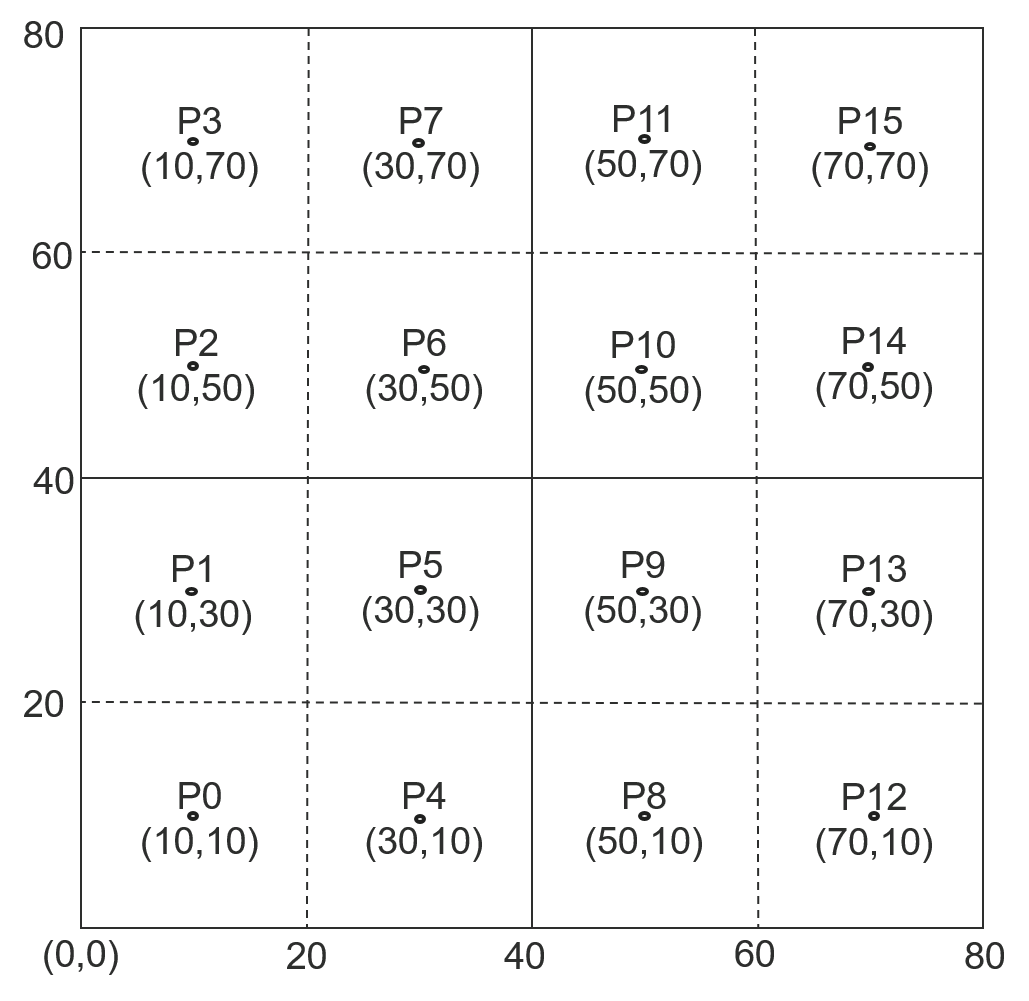
\includegraphics[width=0.7\textwidth]{pix/p10}
    \caption{arrangement of feature points}
    \label{fig:m1}
\end{figure}
\newline
\par Here we take a look at two different intersection regions, $olap1 = (0,20,40,60)$ and $olap2 = (40,20,80,80)$. When we intersect this overlaps with index it gives the points which resides in the intersection as below.

\begin{table}[h]
    \centering
    \begin{tabular}{ |c|c| } 
     \hline
        p2 & (10,50)\\
        \hline
        p1 & (10,30)\\
        \hline
        p6 & (30,50)\\
        \hline
        p5 & (30,30)\\
        \hline
    \end{tabular}
    \caption{Output with overlap region 1}

    \begin{tabular}{|c|c|}
        \hline
        p14 & (70,50)\\
        \hline
        p15 & (70,70)\\
        \hline
        p13 & (70,30)\\
        \hline
        p9  & (50,30)\\
        \hline
        p10 & (50,50)\\
        \hline
        p11 & (50,70)\\
        \hline 
    \end{tabular}
    \caption{Output with overlap region 2}
\end{table}
\par As we can see, quadtree can extract and list features from area of interest.

%-------------------------------------------------------------------------------%
\section{Ranking based on Quality Preferences}

There are other type of advanced ranking mechanism available when more data about the features to be indexed is available. One of such method is ranking based on quality preferences. In this method, we look at some overall mathematical quality of spatial neighbourhood to determine the quality of the feature. There can be more than one methods to rank spatial neighbourhood based on mathematical functions.
\newline
\par For example, If one wants to buy a house, he considers many factors besides the attributes of the house itself. Although qualities of house such as area, no of rooms and price are crucial factors, other neighbourhood qualities such as distance from good quality restaurants or availability of general hospital are also an important factor. One always wants to have his or her home nearby good facilities like hospitals, restaurants and cinemas. The quality of each of this feature in the spatial neighbourhood of house is the determining factor while considering to buy the house.
\newline
\par Quality of each of the facilities is also an important factor. This is why we have defined spatial neighbourhood quality as a parameter of quality of each type of facility and not the quantity of feature types. One can also use the total sum of quality of all features in spatial neighbourhood. That will give the quantitative measure of quality features in the neighbourhood. For example, if there are more number of features that are low in quality, that neighbourhood can still be ranked higher than a spatial neighbourhood where there are less number of high quality features. Other types of mathematical measures can also be employed such as average quality of each feature or sum of average quality of each feature type in spatial neighbourhood. 

\subsection{Algorithm}
This algorithm ranks the quality of spatial neighbourhood for every feature to be ranked. Set of input features with information about other qualitative features are required for this purpose. We also need to set neighbourhood radius for examining spatial neighbourhood. The algorithm takes the input and finds the ranking of the input features. To do this, it first scans the spatial neighbourhood around each features. This is done by creating a bounding box of specified radius around the feature point. We find all the qualitative features in the spatial neighbourhood and find the maximum quality of each type of feature from the neighbourhood. The sum of each type of quality feature gives a score to a particular input feature. Input feature are ranked by decreasing order of their neighbourhood score.
\newline
\begin{algorithm}[h]
    \caption{\em Ranking based on quality preferences }
    \textbf{Input:}\\
    \indent \textit{features}: Set of spatial point features  \\
    \hspace{1cm} \textit{qualitative\_features}: Set of features with quality\\
    \textit{radius}: Spatial neighbourhood radius\\
	\textbf{Output:}\\ 
	\hspace{1cm} Ranking of input features based quality of spatial neighbourhood
	
	\algnewcommand{\Initialize}[1]{%
        \State \textbf{Initialize:}
        \Statex \hspace*{\algorithmicindent}\parbox[t]{.8\linewidth}{\raggedright #1}
        \newline
    } 
	
	\begin{algorithmic}[1]
	    \Initialize{
	        \State $boundary\_box \gets $ Create bounding box based on radius and feature bounding box
	        
	    }
	    \FOR{$feature$ in $features$}
	        \State $qfeatures \gets $ Get all $qualitative\_features$ in the $boundary\_box$ of $feature$
	        \State $feature.quality \gets 0$
	        \FOR{$qtype$ in $qualitative\_feature$ types}
	            \State $qtype.quality \gets$ extract maximum quality for the $type$ in $bondary\_box$
	            \State $feature.quality \gets feature.quality + qtype.quality $
	        \ENDFOR
	    \ENDFOR
	    \State $ranked\_list \gets features$ ranked by $feature.quality$
	    \FOR{$feature$ in $ranked\_list$}
	        \State $Display(feature)$
	    \ENDFOR
	\end{algorithmic}
\end{algorithm}

\subsection{Example Scenario}
\par In our example, we have taken four feature points to rank. They are $feature0(20,20)$, $feature1(20,60)$, $feature2(60,20)$ and $feature3(60,60)$. There are two types of neighbourhood features that we are interested in called box features and star features. Locations of star features are x1(10,70), x2(30,70), x3(10,30), x4(30,30), x5(10,10) and x6(50,30). Locations of box features are y1(10,50), y2(50,70), y3(70,70), y4(70,50), y5(70,30), y6(70,10). Quality of each box and star features are shown in the figure \ref{figure:quality_ranking}.
\newline
\begin{figure}[h]
    \centering
    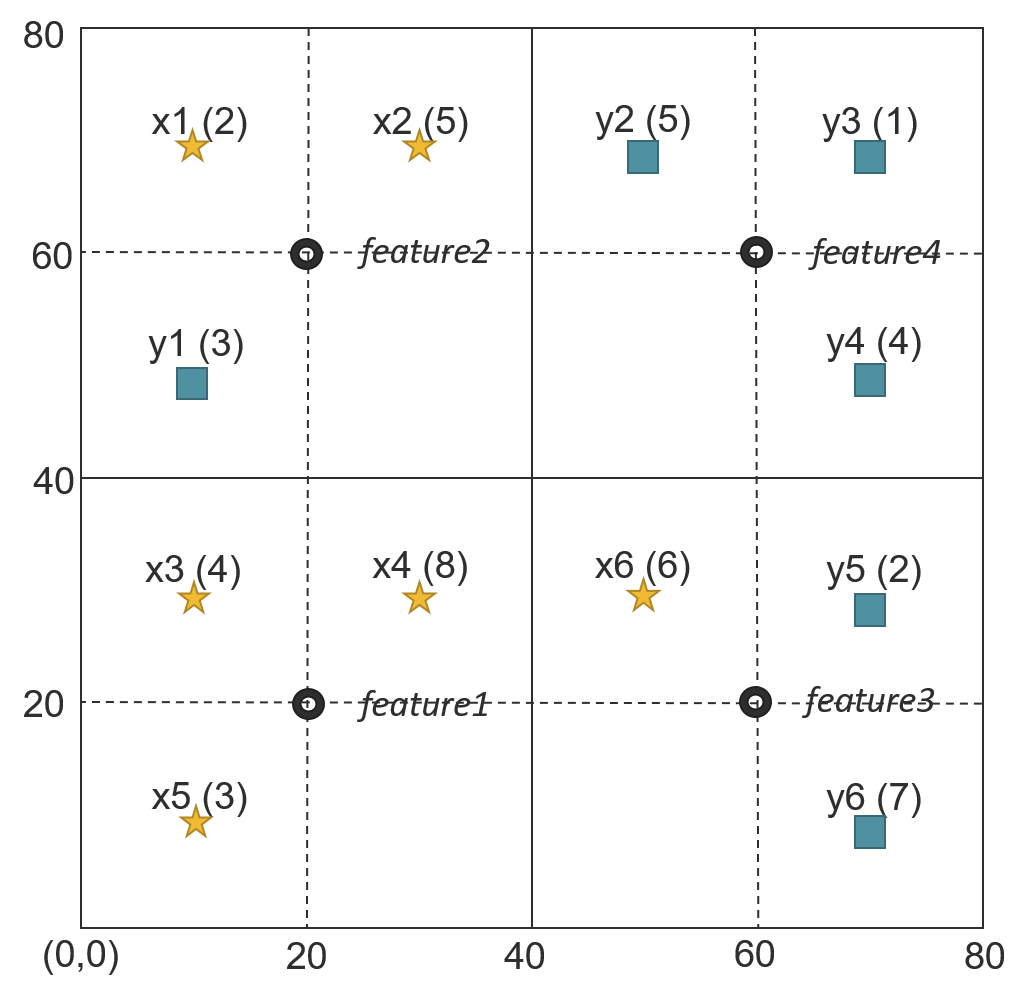
\includegraphics[width=0.7\textwidth]{pix/p11}
    \caption{Ranking by quality preferences}
    \label{figure:quality_ranking}
\end{figure}
\newline
\par In this approach, we first iterate on the feature points, here $feature1, feature2, feature3$ and $feature4$. For each feature we take a neighbourhood region corresponding to it. Here we have taken neighbourhood region to be of 20 distance buffer from the feature point. We find all the relevant features from this buffer and we find maximum quality of star feature and maximum quality of box feature from this buffer. This selected features represents the buffer and in transitive manner the feature itself. We can apply various operations to determine the quality of spatial neighbourhood by applying various mathematical functions on top of it. Here we have chosen the sum function for the demonstrative purposes.
\newline
\par For each feature, the sum of other qualitative features in neighbourhood gives the final score of a feature. The higher the score, lesser the rank. In this example, our final ranking becomes.
\begin{table}[h]
    \centering
    \begin{tabular}{|c|c|}
        \hline
         $Feature$&$Rank$\\
         \hline
         2&13\\
         \hline
         0 & 8 \\
         \hline
         1 & 8\\
         \hline
         3 & 5\\
         \hline
    \end{tabular}
    \caption{Final ranking for the features}
    \label{tab:my_label}
\end{table}
\newline
\begin{figure}[h]
    \centering
    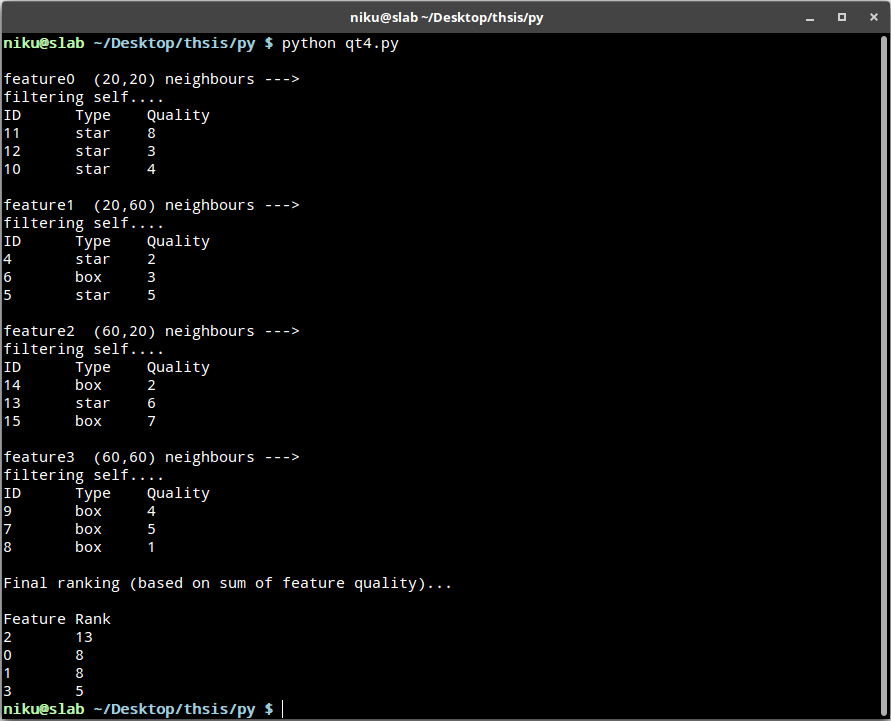
\includegraphics[width=\textwidth]{pix/p12}
    \caption{Features ranked by neighbourhood quality}
    \label{feature_ranking}
\end{figure}
\newline


\chapter{Conclusion and Future Work}

Geo-service portal acts as a underlying framework or foundation for various kind of higher level use cases. Main advantage of this registry service is that we can avail data from various repositories that has been crawled and indexed for others to use. Basic querying facilities can be provided directly on top of registry service. Using geo-spatial crawler we can get the latest geo-spatial data available on the web. Once this data is got from various geo-servers, various kinds of applications can be built on top of that. Building an OGC compliant web service catalog can also be beneficiary as already available software and services can use the registry for various kinds of services with little to no modification of their original code-base.
\newline
\par Geo-service portal can be used for many kind of applications. This applications and use cases include wide variety such as just getting the relevant spatial information for the application to doing in-depth spatial or temporal or spatio-temporal analysis. Other use cases can include finding the spread of the disease on large geographic area. Which of the areas can be affected by flood can also be founded using data from catalog. All this services can work if underlying foundation of catalog service is built.

\section{Contribution of thesis}
Geo-Service portal builds ground work for spatial metadata gathering and publishment. It provides this foundation platform in a modular fashion, such that all of these modules work in a pipeline. Output of one module is feeded as input to other module. This gives independence to update modules irrespective of each other as it has loose coupling.
\newline
\par Spatial web crawler allows to crawl the open web and find existing geo repositories and catalog servers to gather spatial data and store available metadata. This allows better availability of spatial features and data then conventional services.
\newline
\par Spatial catalog server allows us to maintain and publish spatial metadata and provides various OGC compliant services on top of it. This allows not only storage and retrieval of spatial data but also known services and methods attached to retrieval of spatial data and extraction of information from spatial data.
\newline
\par Spatial query orchestration allows retrieval of spatial features in and indexed and ranked manner, which can be useful while working with large number of features. It uses indexing based on quad tree which groups feature based on their proximity from the region of interest. Another advanced method to rank spatial features is by quality preferences, in which quality of feature and it's neighbourhood define the importance of such feature.

\section{Future Scope}
There is significant scope of improvements in the current framework for Geo-service portal as it is designed in a modular way. Extensions and higher level use cases can be provided to any of the modules or newer modules can be added. Some of the advancements to the current features are listed below:
\newline
\par Spatial web crawler module can scrap and crawl other things to make use of other qualities of data the catalog service or repositories that are hosting. This can be useful while ranking the quality of a whole registry with respect to other registries. A score can be provided to crawled registries for the spatial data they contain, size and rarity of the data, by no of times they are referenced and many other such metrics. As spatial data is time driven, catalog service can provide refresh rate, a time after which the catalog service is reloaded to check if their is any change in the data it hosts from the crawled sources. This is useful to find most up to date data from available geo repositories. Analyzing this behavior over a time can also give spatio-temporal behaviour of the data provided by a given repository. For example, spread of city in given range of time and rate of growth can be known. Ranking mechanism can be improved to give scores to repositories and in turn the data crawled from the repositories.
\newpage
\par In today's era, when creating a service reliability, scalability and availability is very crucial things to consider. If the data is hosted on one server and single server architecture is implemented then there might be a high chance of failure on high load. Also the growth of the users and query load on the server cannot be predicted. For this reasons it would be better to consider a cloud based implementation for the above stated architecture. Cloud based implementation for crawler, registry service, and query processor can scale very well in the situations for high load. Cloud based implementation can also be good for availability because on situations of high load, infrastructure can be scaled up to cater the need of high load, in situations of low load the infrastructure can be scaled down to save power and investments. The registry itself can be replicated in the cloud at various geographical places to avail above stated high availability and reliability of the operations. Changes are also be easily and more efficiently done in the cloud because we don't have to shutdown and start the instances again. Cloud instances can be replaced in-place without shutting them down. This ensures versioning can be done of the software and eventual upgradations and roll-out of updates can be provided without hiccups.\\
\par Dynamic deployment of catalog server is the key to achieve high scalability and high availability time. In this approach we can dynamically deploy instances of GeoServer catalog server(s) to accommodate high demand from users. To make it transparent to users, $load\_balancer$ can be used. Similarly we can scale down in case of low demand from users. With these advancements, access control can also be achieved via $load\_balancer$, because it can work as a single point of access for the users. 
\begin{thebibliography}{5}
%%%%%%%%%%% 1
\bibitem{l1}
Sonal Patil, Shrutilipi Bhattacharjee, and Soumya K. Ghosh. \textquotedblleft A spatial web crawler for discovering geo-servers and semantic referencing with spatial features\textquotedblright.\ In \textit{International Conference on Distributed Computing and Internet Technology}, pp. 68-78. Springer International Publishing, 2014.

%%%%%%%%% 
\bibitem{l2}
Li, Wenwen, Chaowei Yang, and Chongjun Yang. \textquotedblleft An active crawler for discovering geospatial web services and their distribution pattern - A case study of OGC Web Map Service\textquotedblright.\ \textit{International Journal of Geographical Information Science} 24, no. 8 (2010): 1127-1147.

%%%%%%%%%%%
\bibitem{l3}
Najork, Marc.\textquotedblleft Web crawler architecture\textquotedblright.\ In \textit{Encyclopedia of Database Systems}, pp. 3462-3465. Springer US, 2009.

%%%%%%%%%%% may not be useful
\bibitem{l4}
Ahlers, Dirk, and Susanne Boll.\textquotedblleft Location-based Web search\textquotedblright.\ In \textit{The Geospatial Web}, pp. 55-66. Springer London, 2009.

%%%%%%%%%%%
\bibitem{l5}
Li, W., C. Yang, D. Nebert, R. Raskin, P. Houser, H. Wu, and Z. Li.\textquotedblleft Semantic-based web service discovery and chaining for building an Arctic spatial data infrastructure\textquotedblright.\ \textit{Computers \& Geosciences} 37, no. 11 (2011): 1752-1762.

%%%%%%%%%%%
\bibitem{l6}
Jiang, Jun, Chong-jun Yang, and Ying-chao Ren.\textquotedblleft A spatial information crawler for opengis wfs\textquotedblright.\ In \textit{Sixth International Conference on Advanced Optical Materials and Devices}, pp. 71432C-71432C. International Society for Optics and Photonics, 2008.

%%%%%%%%%%%
\bibitem{l7}
\textit{http://geopython.github.io/pycsw-workshop/}

\bibitem{l8}
\textit{https://geopython.github.io/OWSLib/}

%%%%%%%%%%%
\bibitem{l9}
Lopez-Pellicer, Francisco J., et al.
\textquotedblleft Discovering geographic web services in search engines\textquotedblright.\
\textit{Online Information Review} 35.6 (2011): 909-927.

\bibitem{l10}
\textit{https://github.com/geoserver/geoserver}

\bibitem{l11}Yiu, Man Lung, Hua Lu, Nikos Mamoulis, and Michail Vaitis.\textquotedblleft Ranking spatial data by quality preferences\textquotedblright.\ \textit{IEEE Transactions on Knowledge and Data Engineering} 23, no. 3 (2011): 433-446.

\bibitem{l12}
Hjaltason, Gisli, and Hanan Samet.\textquotedblleft Ranking in spatial databases\textquotedblright.\ In \textit{Advances in Spatial Databases}, pp. 83-95. Springer Berlin/Heidelberg, 1995.

\bibitem{l13}
\textit{https://github.com/karimbahgat/Pyqtree}

\bibitem{l14}
Paul, Manoj, and S. K. Ghosh.\textquotedblleft An approach for service oriented discovery and retrieval of spatial data\textquotedblright.\ In \textit{Proceedings of the 2006 international workshop on Service-oriented software engineering}, pp. 88-94. ACM, 2006.

\bibitem{l15}
Nogueras-Iso, Javier, Francisco Javier Zarazaga-Soria, Ruben Bejar, P. J. Alvarez, and Pedro R. Muro-Medrano.\textquotedblleft OGC Catalog Services: a key element for the development of Spatial Data Infrastructures\textquotedblright.\ \textit{Computers \& Geosciences} 31, no. 2 (2005): 199-209.

\bibitem{l16}
Jones, Christopher B., Alia I. Abdelmoty, David Finch, Gaihua Fu, and Subodh Vaid.\textquotedblleft The SPIRIT spatial search engine: Architecture, ontologies and spatial indexing\textquotedblright.\ In \textit{International Conference on Geographic Information Science}, pp. 125-139. Springer Berlin Heidelberg, 2004.

\bibitem{l17}
Lopez-Pellicer, Francisco J., Aneta J. Florczyk, Ruben Bejar, Pedro R. Muro-Medrano, and F. Javier Zarazaga-Soria.\textquotedblleft Discovering geographic web services in search engines\textquotedblright.\ \textit{Online Information Review} 35, no. 6 (2011): 909-927.

\end{thebibliography}

%%%%%%%%%%%
% \bibitem{latexcompanion8}
% Suakanto, Sinung, et al.
% \textit{Building crawler engine on cloud computing infrastructure.}
% Cloud computing and social networking (ICCCSN), 2012 international conference on. IEEE, 2012.

% \chapter{Introduction}

The Internet is a major source of all information which includes news as well.It is also the next important source of information after television as per \cite{kohut2008internet}.Nowadays, social media sites have had an impact on news journalism.People use primarily social media to interact with their friends and family but also to share news \cite{java2007we}.This is done to convey updated information to people around them.The ease of use of social media has made this information flow much faster than ever before.In emergency and disaster situations,Twitter has proven to be great aid \cite{vieweg2010microblogged}.
\\
\par
Online social networks allow users to post any information that the users intends to convey to others.Due to the advent of social networks, anyone can express their views on any of the available platforms.This facility allows information to be propagated in real time rapidly to a large audience.This helps in certain situations where other media such as news require more time to convey the same information.But along with the fast pace of information diffusion in social networks comes the problem of the reliability of the information.Due to the open and uncontrolled nature of online social networks anyone can post any information either deliberately or inadvertently without verifying the authenticity of the facts involved.This kind of information can lead to the spread of rumors in the network.A rumor is considered as a statement whose truth can be verified at the current instant of time given all the relevant evidence.Rumor also has a component which is controversial i.e. some people may not accept the fact directly and will raise questions about its correctness.Rumors can cause incorrect facts to be propagated and may cause panic in the population.\\
\par
Twitter is a online social network where user can post small messages called Tweets which can contain up to 140 characters.Some users also retweet - which is a repost or forward of a tweet by another user. It is indicated by the characters RT.The ubiquity, accessibility,speed and ease-of-use of Twitter have made it an invaluable communication tool.People turn to Twitter for a variety of purposes, from everyday chatter to reading about breaking news.Users can explicit write new messages or they can re-tweet tweets which are written by other Twitter users.Due to the re-tweet facility available,the rate of information propagation is increased in some cases as some tweets will become viral and many users will re-tweet it.The increase in the number of smart phones and the number of people using those to write/read tweets has exploded the amount of information being generated.Detection of rumors plays an important role in such context.\\
\par
Before we proceed with the explanation of our algorithms for rumor detection and verification,we need to examine what exactly a rumor is. We state a rumor to be an unverified assertion that starts from one or more sources and spreads over time from node to node in a network.On Twitter,a rumor is a collection of tweets which is unverifiable which are tweeted and then re tweeted subsequently to form an cascade as the information flows through the Twitter network.Rumors can be concluded in may ways - it may either turn out to be true, false or remain uncertain till a certain verifiable account of information is available.There can be many rumors about some specific object in various context.The final outcome of one rumor with regards to a specific object can help to reach a decision to decide the other rumor in some other context.Hence it is important to identify the exact topic of the rumor which is being propagated through the network. 
\\
\par
Given the huge rate at which tweets are generated,it is impossible for any human to track down all the rumors that are currently present.There is therefore a need for an automated tool which can provide the list of potential rumors.As this list will be comprehensible by a human,the output provided by such a tool will be helpful to take corrective actions against the rumor.For example,if the fact in a rumor has an relevant authority, the authority can either vouch for or disapprove the rumor using the same social network.This will limit any false rumor from propagating to a large audience thereby limiting the spread of misinformation caused by it and other effects it may cause in the population. \\
\par
\clearpage
The overall thesis is organized as follows -
\begin{itemize}
	\item In Chapter 2, we include a survey of related literature.
	\item In Chapter 3, we present our methods for the tweet retrieval and tweet filtering. 
	\item In Chapter 4, we present the tweet clustering results and the analysis of the distinct properties of rumors.
	\item Finally, we conclude the work in Chapter 5 and provide directions for future research.  
\end{itemize}


% \newpage
% \chapter{Review of Literature} 
There has been significant research on information diffusion in the context of social networks.A broad discussion of these is available in \cite{guille2013information}.In this article, they have analyzed multiple methods related to information diffusion analysis in online social networks, ranging
from popular topic detection to diffusion modeling techniques, including methods for identifying influential spreaders.They have indicated that bursts are a good signal to identify popular topics.Information diffusion may be modeled using both graph and non graph based methods.There are many ways to identify influential spreads in a network including pure topological approaches, such as k-shell decomposition or HITS.
It provides various ways to model information spread in a social network.The work done here does not deal the information content that is being flowed through the network.To detect rumors,we not only need the information related to the information diffusion but also the content of the information that is being propagated. \\
\par 
The work done in \cite{castillo2011information} is the most extensive work related to the credibility of tweets posted on Twitter.They first build a dataset of tweets using detection of bursts within Twitter.Using manual annotators the tweets are divided into bins corresponding  to the amount of confidence that the annotator has in the tweet.They extract user,message,topic and propagation based features which is then used to build a classifier.Then supervised learning is used to identify the set of tweets of unverified information.They also perform best feature selection to determine the features which have maximum impact and thus play a crucial role in the classifier that is built.They emphasize the importance of validation of credibility of the information posted on Twitter as a safeguard for inexperienced users who can be misled by incorrect information. 
\\
\par
The approach used in \cite{qazvinian2011rumor} attempts to formulate the model for rumor detection and then build a classifier out of it.They divide their work into two parts namely-rumor retrieval and belief classification.Rumor retrieval step deals with the task of finding a set of controversial tweets.The next step i.e. belief classification finds the set of users who suspect the statement to be rumor and raise question on it.They annotate a set of tweets as 1 or 0 depending upn whether a user believes whether it is a rumor or not.Using these annotated tweets,they extract features from the tweet dataset of different types such as content,network and some Twitter specific features.They manually annotate a set of tweets and then train a classifier to predict whether a new tweet contains a rumor or not.The work is mainly targeted to retrieve a set of related rumors in the dataset but it does not detect new types of rumors that are not contained in the training dataset.\\ 
\par
The work as described above takes into account only the temporal and linguistic properties of the Twitter dataset.The work done in \cite{kwon2013prominent} is the first work to distinguish the temporal properties of rumor v/s a non rumor dataset.They have successfully demonstrated that temporal features have greater impact in decision of a rumor tweet.Rumors show bursty fluctuations over time unlike other random tweet chatter occurring over Twitter.The difference in spike behavior has been demonstrated as a good signal to differentiate the non rumor tweets.The work done in this thesis thus extends this notion and works primarily on temporal properties.This work has done the relative ranking of importance of various features and also mentioned which features dominate the decision to formulate a rumor. 
\\
\par
Another work done in \cite{sun2013detecting} uses Sina Weibo rather than Twitter as dataset due to the large number of users compared to Twitter.In addition to the standard linguistic and user features used in the previous work they have used multimedia features - one of them which is timespan.The timespan is calculated based upon the posted date of the new microblog and the posted date of the old image. If a microblog does not contain any picture, then value of timespan to be 0. If the timespan between the text and the picture is bigger than the threshold, then the value is 1.Otherwise the value is 2.The point to conclude is that rumors mostly contain images which are earlier posted on the Internet.Thus this work also depicts the importance of temporal properties when judging for a rumor.
\\
\par
The work done in \cite{zhao2015enquiring} propose a real-time rumor detection procedure that has the five steps.The algorithm first finds enquiry tweets using a set of regular expressions .This set of tweets are called as signal tweets.Then they use Jaccard similarity to cluster these signal tweets.They calculate the Jaccard similarity by taking 3-ngrams of each tweet. Jaccard similarity is a commonly used indicator of the similarity between two sets.It is calculated as follows.

\begin{equation}
Jaccard(a,b)= \frac{|ngram(a) \cap ngram(b)|}{|ngram(a) \cup ngram(b)|}
\end{equation}

They find the the most frequent and continuous substrings(3-grams that appear in
more than 80\% of the tweets) and output them in order as the summarized statement.Then they use this summary statement to compare with each of the tweets which are not signal tweets.This is done so that more tweets are included in the cluster which will help to build a better classifier.This is necessary because the signal tweets detected is very less compared to the non signal tweets.Using statistical features of the clusters that are independent of the statements content, they rank the candidate clusters in order of likelihood that their statements are rumors.\\
\par


% \newpage
% \chapter{Information Extraction}

			\section{Problem Definition}

			\par
			We first define what constitutes a rumor.As per \cite{difonzo2007rumor} a rumor is defined as -
			\begin{center}
					A rumor is a controversial and fact-checkable statement.
			\end{center}
			We make certain observations related to the above definition:-
			\begin{itemize}
				\item Fact-checkable: It means that one can verify the correctness given the concrete evidence for the same.Statements for which truth value will be determined in future are not included.
				
				\item 
				Disputable: People will not accept and will question the belief discussed in the information.
			\end{itemize}
			Any statement will includes a reference to a statement which has the above 2 properties can be also considered as rumor.
			\\
			\par
			Most of the work done above in the context of rumor detection considers the data using only it's lexical and syntactic features.For example, work done in \cite{zhao2015enquiring} treats tweets using the Bag-of-Words model to calculate the tweet similarity.For the problem of rumor detection it is necessary to identify the subjects that the rumor is spreading.Using the Bag-of-Words model,we don't have any sufficient information to identify the subject(s) that is/are being discussed  in tweet data involved. The accurate subject identification of tweets however is a challenging task since the limited number of tokens in a post often implies a lack of sufficient	contextual information.There is a certain need to analyze the problem by identifying its semantic features.\\
		
			\par
			The problem is formulated as follows.Given a set of tweets,we need to group them into rumor clusters.Each cluster is identified by the subject discussed in the rumor.Then we enrich the semantic context of each cluster by extracting subjects contained in them.After this step,rumor analysis of each cluster is to be done to indicate the probability that it represents a rumor.The subjects which are extracted using Part-of-Speech tags are used to extract semantic information from the tweets.The semantic information is then used to cluster the tweets as a similarity measure.
			\\
			\par
			The below diagram shows the overall flow of the working of the system proposed.\\
			\begin{figure}[H]
				\centering
				\begin{minipage}{1\linewidth}
					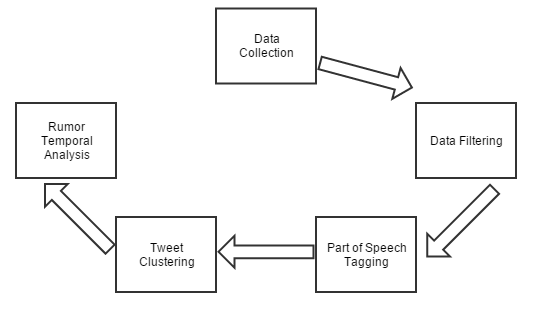
\includegraphics[width=\linewidth]{images/block.png}
					\captionof{figure}{Flow diagram}
					\label{img1}
				\end{minipage}
			\end{figure}
			
		\clearpage	
			
		\section{Terminology}
		
		We first define some Twitter specific terms that will be used:-
		
		\begin{itemize}
			\item Tweet - Each message written on Twitter is called a tweet.
			\item Feed - A feed is any constantly-updating list of tweets or other updates, usually sorted chronologically with the most recent updates appearing at the top.
			\item Follower - On Twitter, you follow another user to see his or her updates on your Twitter home page.
			\item Mention - Twitter allows user to mention other user in a tweet using @ symbol.
			\item Hashtag - Using \# symbol a user can enrich the subject being discussed in the tweet.  
			\item Retweet - Using retweet we can make someone else's tweet appear in stream of our followers.
		\end{itemize}	
					
		\section{Data Collection}
		\par
		The tweets are collected using the Twitter Streaming API which provides 1\% sample of the real-time tweets.We use the data available from Twitter for the month of July 2015.Given the huge volume of the data,the tweets are stored into a NoSQL MongoDB database in JSON format.A NoSQL (originally referring to "non SQL" or "non relational") database provides a mechanism for storage and retrieval of data which is modeled in means other than the tabular relations used in relational databases.Storing in the JSON format allows the meta-data to be updated over the time to add new features to the tweet data as well as enable efficient retrieval of large amount of data.The JSON data is then exported to HDFS for Map-Reduce operations on this large scale data.
		\\
		\par
		The current dataset is limited to tweets which are written only in the English language.The information contained in the tweet meta-data is used to select only the English tweets.The data is filtered to remove the tweets which are written in multiple lines.This is done to facilitate processing on HDFS which considers one line as a single record.As the number of tweets having multiple lines is a small fraction of the total tweets,it is assumed that removing these does not impact the correctness of further operations.The tweets were also more or less evenly divided between each day of week, with each day having somewhere between 14\% and 15\% of the tweets. Similarly, the tweets were almost evenly divided between each hour, with each having somewhere between 3\% and 5\% of the tweets.The overall distribution of the tweets posted per day for the month of July 2015 of the 1\% dataset is shown below. 
		
			\begin{figure}[H]
				\centering
				\begin{minipage}{.7\linewidth}
					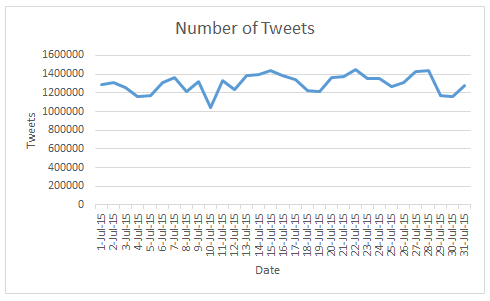
\includegraphics[width=\linewidth]{images/num_tweets.png}
					\captionof{figure}{Number of Tweets}
					\label{img_nt}
				\end{minipage}
			\end{figure}

		\section{Data Filtering}
		\par The set of tweets collected is divided into two sets - signal tweet and non signal tweet.Signal tweets are those which contain enquiry pattern such as "really?","is it true" as identified in \cite{zhao2015enquiring}.These signal tweets are used as signal element to identify a rumor.All others tweets other than enquiry tweets are collected into the non signal tweet set.
		This is done to identify the first set of signal that may be used to indicate that a tweet may be a rumor.As per figure \ref{img_nt} we have seen that the number of tweets per day is very large and the average is around 1.3 million tweets per day.To process such data,we need certain type of distributed computation to scale up the processing time and get results within a minimum stipulated time.We have used Hadoop framework to process this "big" data.Hadoop used HDFS as the filesystem to store files i.e. the tweet data in current context.The Map-Reduce framework is then used to filter the tweets wherein the work is distributed to multiple machines in the cluster and partial results are then aggregated to form a unified dataset of filtered tweets.  
		
		
		\section{Part-Of-Speech Tagging}
		A Part-Of-Speech Tagger (POS Tagger) is a piece of software that reads text in some language and assigns parts of speech to each word (and other token), such as noun, verb, adjective.The current approach uses POS tagging to extract syntactic features from each tweet rather than the lexical model used in previous works.The syntactic features will be later used to derive semantic information about each subject discussed in the tweet cluster.		Standard POS tagging tools are used to extract POS tags from sentences in long documents.Tweets are online conversations which are short and it's word usage is different than of long text documents.Standard POS tagging tools are trained on data sets of large words,hence do not work on tweets.A specialized tool for tweets is needed for perform POS tagging efficiently.So an existing efficient and specialized Twitter POS tagging tool \cite{gimpel2011part} is used for extracting  POS features.The tool decomposes the tweets into various components such as proper noun,common noun,verb,adjective,adverb and interjection.Some Twitter specific POS tags such as hash tag,user-mention,URL and emoticon are also retrieved.

		\par For example, the following tweet
		\begin{center}
		 "RT @brownjenjen : Ben Affleck denies affair rumors
		\#rumor http://t.co/qwrfe"
		\end{center} 
		\par is decomposed in POS tags as follows:-
		
		
\begin{table}[H]
	\centering
	\begin{tabular}{@{}|l|l|@{}}
		\toprule
		RT                & Re-tweet         \\ \midrule
		@brownjenjen        & At-mention       \\ \midrule
		:                 & Discourse marker \\ \midrule
		Ben               & Proper Noun      \\ \midrule
		Affleck           & Proper Noun      \\ \midrule
		denies            & Verb             \\ \midrule
		affair            & Common Noun      \\ \midrule
		rumors            & Common Noun      \\ \midrule
		\#rumor           & Hashtag          \\ \midrule
		http://t.co/qwrfe & URL              \\ \bottomrule
	\end{tabular}
	\caption{Tweet Part-of-Speech Tagging}
	\label{my-label}
\end{table}




\section{Tweet Clustering}
This process involves dividing a set of tweets into subsets, where elements in each subset are considered related by some similarity measure.It is very rare that tweets which contain different subjects will contain any similarity on a semantic basis.Using a string similarity measure may lead  to a spurious similarity for tweets even if they are not related.So the current approach avoids use of a string similarity measure and instead represents each tweet by proper nouns and URLs contained in it.These are obtained by the POS tagging step done earlier.The number of similar proper nouns and URLs are used a measure of similarity.
\\
\par
Each tweet is added as a node in the graph.An edge is added between two tweets only if they represent some common subject i.e. proper noun/URL.The weight of the edge determines the degree of similarity which is number of matching POS tags.Any POS tag that is matched is assigned a score of 1.The edge accumulates the scores of individual matching POS tags.An undirected graph of tweets is built by including an edge joining any tweet pair with a similarity score of at least 2.
This is done to ensure that the rumors clusters are accurate.The accuracy of the clusters is determined by the subject discussed within them but also by its context.It may happen that one subject is being discussed with two different contexts in the same temporal dimension.For example,"Obama" may be discussed related to two other subjects such as "nuclear deal" and "war".It is necessary to form two candidate rumor clusters separately for each of them.By adding an edge only when similarity score is 2,such dataset will have two clusters - one related to "Obama" POS tags with "nuclear deal" related POS tags and the other with "Obama" POS tags with "war" related POS tags.This splitting of clusters also allows each cluster to be analyzed independently of each other.This improves the coherent quality of each cluster as each of them has the exact context discussed and does not mix tweets with other context.      
\\
\par
A connected component in an undirected	 graph is a group of vertices, every pair of which are reachable from each other through paths.The connected components in such a graph will contain the tweet cluster which discuss a common subject.Next,we calculate the summary features of each cluster by including the POS tags which occur in more than 25\% of the tweets in the cluster.This step ensures that only the subjects that are actively being discussed will be brought in the tweet cluster summary.The summary statement consisting of POS tags is now compared with each tweet in the non signal cluster set to increase the cluster size.	  
\\
\par
The entire algorithm is outlined below.

\begin{algorithm}[H]
	\caption{\em Tweet clustering algorithm from Part-of-Speech tags - Single Day }
	\textbf{Input:} Raw tweets from Twitter 1\% sample dataset \\
	\textbf{Output:} Clusters of candidate rumors 
	%\begin{minipage}{\linewidth}
	\begin{algorithmic}[1]	 	
		\FOR{ All tweets in dataset }
		\IF{Tweet contains enquiry pattern} 
		\STATE{Add tweet to signal tweets set} 
		\ELSE 
		\STATE{Add tweet to non signal tweets set} 
		\ENDIF
		\ENDFOR    
		
		\FOR{ All tweets in the signal set}
		\STATE Add tweet as node in graph 
		\STATE	 Extract Part-Of-Speech tags from each tweet 
		\STATE	 Assign proper noun and/or URL as features for each tweet
		\STATE	 Compare with rest of the signal tweets
		
		\IF{Number of features matching is greater than or equal to 2} 
		\STATE{ Add edge between the tweets }
		\ENDIF
		\ENDFOR
		\STATE Get connected components from the graph
		\IF{ Size of connected component is less than 2 }
		\STATE Discard connected component
		\ELSE
		\STATE Consider connected component as a candidate rumor cluster
		\ENDIF
		\FOR { Each candidate cluster}
		\FOR { Each tweet in the cluster}
		\IF {Feature of tweet is contained in more than 25\% percent of the tweets in the cluster}
		\STATE Add feature to summary feature set of the cluster 
		\ENDIF
		\ENDFOR
		\ENDFOR
		\algstore{testcont} 
	\end{algorithmic}
	\addtocounter{algorithm}{-1}%% <===
\end{algorithm}

\begin{algorithm}[H]
	\caption{\em Tweet clustering algorithm from Part-of-Speech tags - Single Day}
	\begin{algorithmic}[1]
		\algrestore{testcont}  
		\FOR { Each candidate cluster}
		\FOR { Each tweet in the non signal tweets}
		\IF{ Number of matching features between candidate cluster summary and the non signal tweet is greater than or equal to 2 }
		\STATE Add tweet to candidate rumor cluster 
		\ELSE
		\STATE Discard the tweet for further processing 
		\ENDIF 
		\ENDFOR
		\ENDFOR 
	\end{algorithmic}
	%\end{minipage}
\end{algorithm}

		\section{Results}
		To process such large data in a distributed manner, the algorithms were executed out on a Hadoop cluster having 15 nodes.The data filtering results for signal tweets that were carried out are explained below.
		
		\begin{figure}[H]
			\centering
			\begin{minipage}{.7\linewidth}
				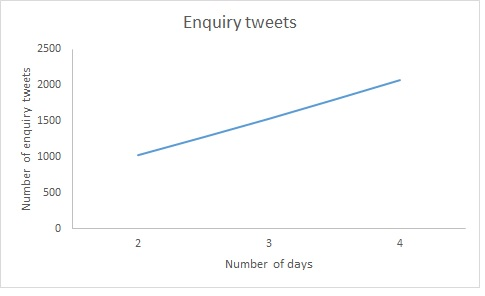
\includegraphics[width=\linewidth]{images/result1new.jpg}
				\captionof{figure}{Days vs Signal Tweet Size}
				\label{img1}
				\end{minipage}
		\end{figure}
		
		Figure \ref{img1} shows the number of enquiry tweets collected over days.The number of enquiry tweets is directly proportional to the size of the dataset.This concludes that everyday there exists a proportion of the users whose post enquiry tweets.This linear increase also proves that each day  there is more or less a fixed amount of Twitter chatter which consists of the portion of signal tweets.
				
		\begin{figure}[H]
					\centering
					\begin{minipage}{.7\linewidth}
						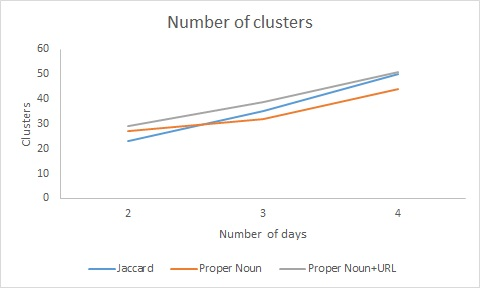
\includegraphics[width=\linewidth]{images/result2new.jpg}
						\captionof{figure}{Number of clusters}
						\label{img2}
						\end{minipage}
		\end{figure}
		
			Figure \ref{img2} shows that the number of clusters we get using tweet similarity measure as Jaccard distance is similar to the number of clusters we get using the proper noun POS tweet similarity measure.The proper noun+URL POS tweet similarity measure provides the best performance in all cases.Thus,we stick to this measure for all further operations.
						
		\begin{figure}[H]
							\centering
							\begin{minipage}{.7\linewidth}
								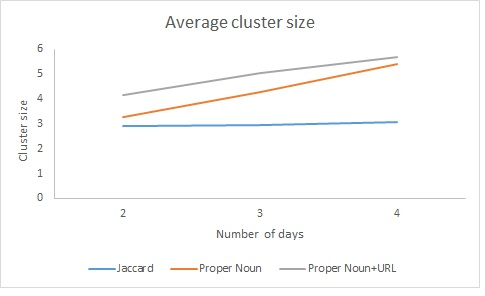
\includegraphics[width=\linewidth]{images/result3new.jpg}
								\captionof{figure}{Average cluster size}
								\label{img3}
								\end{minipage}
		\end{figure}
		
		Figure \ref{img3} shows the average cluster size for varying amount of tweet data.The average cluster size does not increase for Jaccard distance as larger datasets containing the same concept contains tweets which will contain diverse words. The diversity of the words involved in larger datasets will reduce the Jaccard similarity between tweets leading to small clusters being formed.When using POS tags, diverse words wont affect the result as they are not taken into account when determining the cluster similarity.In fact more the data, POS tag approach will lead to bigger clusters being formed.If we add URLs extracted from the POS tag in addition to proper noun, we get more bigger clusters as many tweets which contain a rumor which share a URL which contains more information about the fact being claimed.
								
		\begin{figure}[H]
									\centering	
									\begin{minipage}{.7\linewidth}
										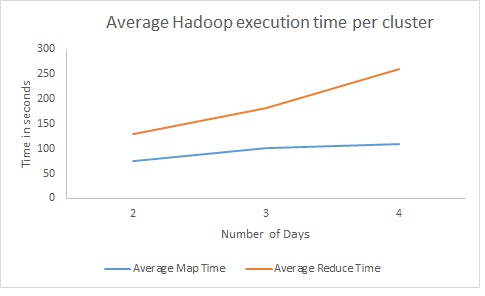
\includegraphics[width=\linewidth]{images/result4new.jpg}
										\captionof{figure}{Hadoop execution time}
										\label{img4}
										\end{minipage}
		\end{figure}
										

		While increasing the dataset shows improvement in the number of clusters and the average cluster size as shown in the Figures  \ref{img2} and \ref{img3},the corresponding time required to process the non signal tweets to be assigned to a signal cluster also increases as shown in figure \ref{img4}.In fact,the time required for Reduce operation starts to increase non-linearly.This metric is crucial when we need to detect rumors as quickly as possible.
		
		\section {Summary}
		
		This chapter has focused on the defining the rumor detection problem in a broad context.The data collection and filtering for the rumor detection purpose has been explained in detail.The semantic information extraction from a single day of Twitter data and its results using Hadoop cluster have been examined.We have also found that Proper Noun+URL Part-of-Speech similarity measure perform the best when clustering the tweets.In the next chapter,we deal with combining the individual Hadoop results of single days and performing rumor analysis.
		
	
% \newpage
% \chapter{Rumor Analysis}

	\section{Combining Overlapping Clusters}	
	
	The earlier results show that increasing data to produce more as well as bigger clusters has a drawback since the time required to process such data increases proportionally with the number of days for which data is taken and thus is not scalable.If we need to see if any rumor is active from last 'n' days, we need to process the 'n' day's data plus the current day's data.Clearly this approach is not scalable as it requires re-computation of the last 'n' days data.An efficient way to do this is store the result for last 'n' days and combine it with the current day's data.By this technique,the unit of data that should be processed can be kept to one day.This each one day's processed data can be combined with earlier data to accurately represent the cluster.
	\\  
	\par 
	The earlier algorithm clusters tweets into candidate rumor clusters for each day to expedite the processing on the Hadoop cluster.But this may lead to disjoint clusters created for each day,where rumors may spread over multiple days.Such rumor clusters which are divided into separate clusters over multiple days must be combined into single cluster so that we can accurately model the cluster for it's temporal and quantitative  characteristics.Such a framework also allows us to add newer data  to existing clusters and check if any of the older rumors still exist or whether they have ceased.
	\\
	\par
	To enable faster processing of clusters,we process only the signal tweets as they form a small portion of the overall tweet volume.Jaccard distance is used to calculate the distance between two tweets.Prior to clustering the tweets, the tweet data is processed using standard text preprocessing techniques so that the clustering performance is not impacted due to noise in the text data.The tweets are then clustered using hierarchical clustering.Average linking method is used to cluster the tweets is due it's advantages over the other methods.Average-link clustering is a compromise between the sensitivity of complete-link clustering to outliers and the tendency of single-link clustering to form long chains that do not correspond to the intuitive notion of clusters as compact, spherical objects.Average-link clustering merges in each iteration the pair of clusters with the highest cohesion.
	\\
	\par
	The dendogram is cut at height 0.75 which is empirically the best value among all other values at which cut is done.Such a clustering will still lead to large number of small clusters.This is primarily due to the sparsity of the words contained in the tweets and the 140 character limit of each tweet.But these small clusters are indeed disjoint components of a bigger cluster.The algorithm 1 produces a list of clusters along with its summary features.These summary features can be used as semantic features to combine the clusters.For example, if a cluster obtained using the algorithm 2 contains summary features as f1,f2..fn, we can search other clusters where tweet has summary feature f1,f2,..fn.If such a tweet is found in another cluster of algorithm 1,the tweet and all other tweets containing in it's cluster are combined with the original cluster.This process is carried out transitively until no cluster produced by algorithm 1 can be further merged into a cluster produced by algorithm 2.	
	\\
	\par
	The entire algorithm is outlined below.
	
	\begin{algorithm}[H]
		\caption{{\em Tweet clustering algorithm - Multiple days}}
		\textbf{Input:} Signal tweets with summary features  from output produced by Algorithm 1 \\
		Non Signal tweets with summary features  from output produced by Algorithm 1 \\
		\textbf{Output:} Clusters of candidate rumors spanning multiple days \\ 
		\begin{minipage}{\linewidth}
			\begin{algorithmic}[1]	 	
				\FOR {All tweets in input-signal-tweets}
				\STATE Remove punctuation from the tweet
				\STATE Remove all the extra white space between words
				\STATE Convert all the words in tweet to lowercase
				\STATE Remove stopwords from the tweet	
				\ENDFOR
				
				\FOR {Tweet 'a' in input-signal-tweets}
				\FOR {Tweet 'b' in input-signal-tweets}
				\STATE Calculate word-level Jaccard between tweet 'a' and tweet 'b' and store the result in the distance matrix at location distance[a][b]
				\ENDFOR
				\ENDFOR
				
				\STATE Use hierarchical clustering using average linkage to produce the dendogram using the distance matrix
				\STATE Cut the dendogram at height determined empirically to determine the clusters
				\STATE Rank the clusters based on decreasing order of their size
				\FOR{ Each cluster 'c2' produced by algorithm 2}
				\STATE Extract unique summary features contained in the cluster
				\IF { A tweet in cluster 'c1' produced by algorithm 1 contains these summary features }
				\STATE Combine cluster 'c1' with 'c2'
				\ENDIF
				\STATE Repeat above steps until no cluster 'c1' can be further merged into cluster 'c2'
				
				\FOR{All input-non-signal-tweets}
				\IF { tweet summary matches to any unique summary features contained in the cluster }
				\STATE Add non-signal tweet to cluster
				\ENDIF	   
				\ENDFOR
				\ENDFOR
			\end{algorithmic}
		\end{minipage}
	\end{algorithm}
	
			 
	\section{Results - Clustering }
	 \begin{figure}[H]
	 	\centering
	 	\begin{minipage}{.7\linewidth}
	 		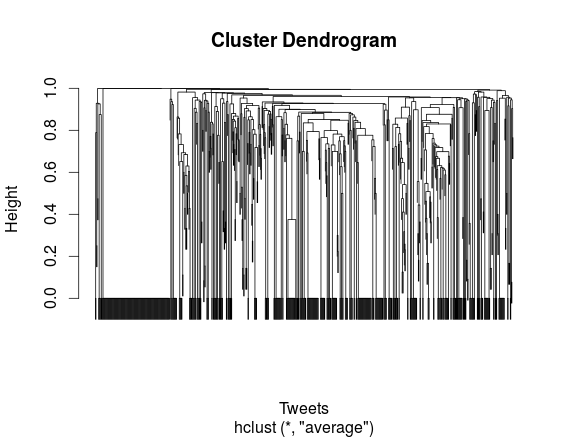
\includegraphics[width=\linewidth]{images/dendogram.png}
	 		\captionof{figure}{Cluster Dendrogram}
	 		\label{img5}
	 	\end{minipage}
	 \end{figure} 	
	 
	 \begin{figure}[H]
	 	\centering
	 	\begin{minipage}{.7\linewidth}
	 		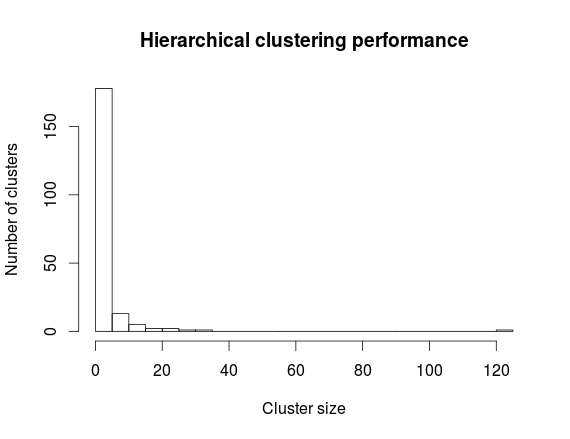
\includegraphics[width=\linewidth]{images/size_of_clusters.png}
	 		\captionof{figure}{Cluster size histogram}
	 		\label{img6}
	 	\end{minipage}
	 \end{figure} 	
	 
	 
	 Figure \ref{img5} shows the dendogram using hierarchical clustering of signal tweets using word level Jaccard distance.When this tree is cut at height 0.75, we get the clusters along with their size as shown in figure \ref{img6}.The histogram shows that we have a very large number of small clusters and a very small number of large clusters.Therefore, we need to combine these clusters into larger ones using the common semantic features that were obtained from algorithm 1.
	 
	 \section {Temporal analysis}
	 The next step involves the classification of the rumor clusters as rumor/non-rumors.The first focus is on the temporal aspects of the cluster.Other quantitative properties of the rumor will be explored later.We examine the rate of growth of tweet volume in a tweet cluster as a feature to classify the cluster.To calculate the rate of growth,the tweets are first sorted according to their tweet date.A new attribute rank 'i' is added to each tweet indicating that it is the 'i'th ranked tweet in the cluster according to its create date.A plot of tweet created date vs the rank of tweet in the cluster helps to determine the rate of growth of the tweet volume in the cluster.Analyzing the slope of distinct segments in the plot of can help to distinguish between rumor /non rumor.Each rumor cluster may have different size,hence we perform min-max normalization on the rank attribute to restrict it's values between 0-1 for any range of data.The min-max normalization is carried out as follows,where \begin{equation} x=(x_1,...,x_n) \end{equation} and z is now the ith normalized data :-
	 
	 \begin{equation}
	 z_i=\frac{x_i-\min(x)}{\max(x)-\min(x)}
	 \end{equation}

 \section{Results - Temporal Analysis }
 
 \begin{figure}[H]
	\centering
	\begin{minipage}{.45\linewidth}
		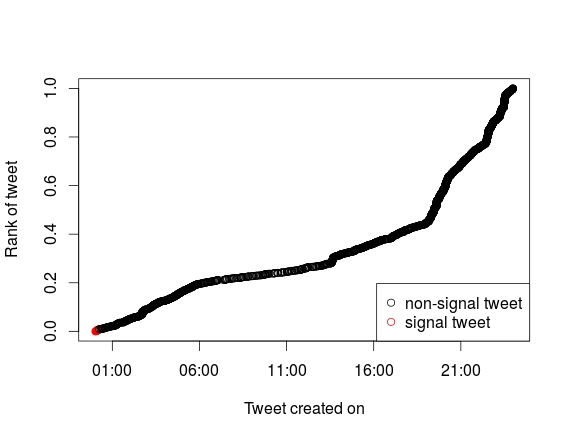
\includegraphics[width=\linewidth]{images/nrumor1.jpeg}
		\captionof{figure}{Tweet Date vs Rank of Tweet - Example 1}
		\label{nr1}
	\end{minipage}
	\hspace{.05\linewidth}
	\begin{minipage}{.45\linewidth}
		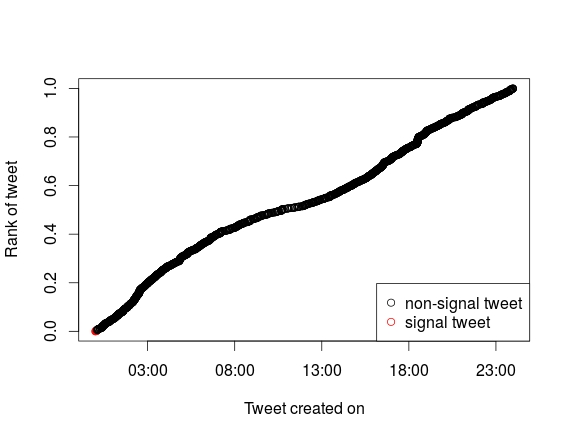
\includegraphics[width=\linewidth]{images/nrumor2.jpeg}
		\captionof{figure}{Tweet Date vs Rank of Tweet - Example 2}
		\label{nr2}
	\end{minipage}
	\centering
	\begin{minipage}{.45\linewidth}
		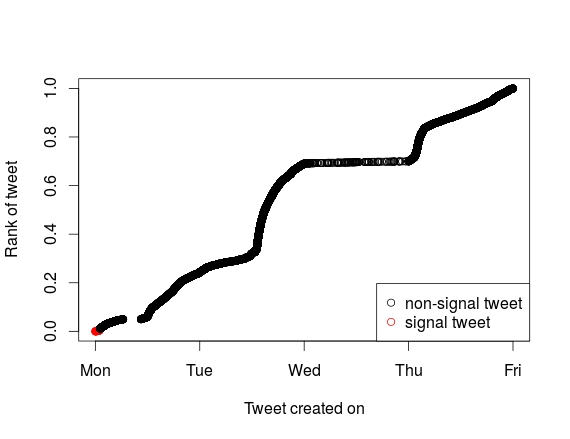
\includegraphics[width=\linewidth]{images/nrumor3.jpeg}
		\captionof{figure}{Tweet Date vs Rank of Tweet - Example 3}
		\label{nr3}
	\end{minipage}
	\hspace{.05\linewidth}
	\begin{minipage}{.45\linewidth}
		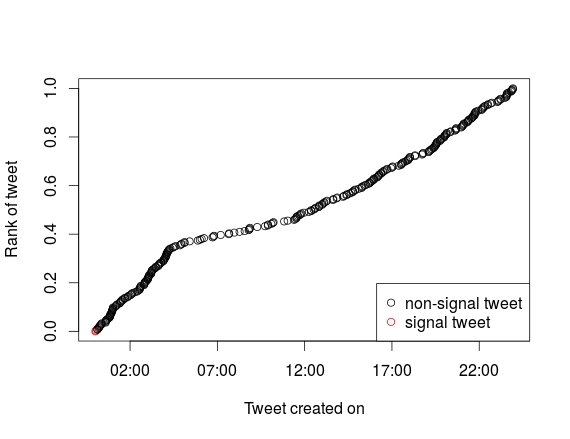
\includegraphics[width=\linewidth]{images/nrumor4.jpeg}
		\captionof{figure}{Tweet Date vs Rank of Tweet - Example 4}
		\label{nr4}
	\end{minipage}
\end{figure}

  In Figure \ref{nr1} we plot the time of tweet v/s the rank of the tweet(i.e. sequence number of the tweet when ordered according to it's create time).
  We can say that the growth of a non-rumor is fairly constant throughout it's lifetime.Since inception till it's end,the number of people posting about it does not deviate much.This can be seen by absence of sparse dots on the plot(we see this pattern in rumor when it's starts to fade away).Due to such behavior,this plot is a non-sparse curve.Owing to less number of distinct segments than a rumor plot,we can fit a linear line through a non-rumor cluster plot with less sum-of-square error than a rumor plot.Figure \ref{nr2},\ref{nr3} and \ref{nr4} show another similar instance of a clusters which do not constitute a rumor. 

 
 
\begin{figure}[H]
	\centering
	\begin{minipage}{.45\linewidth}
		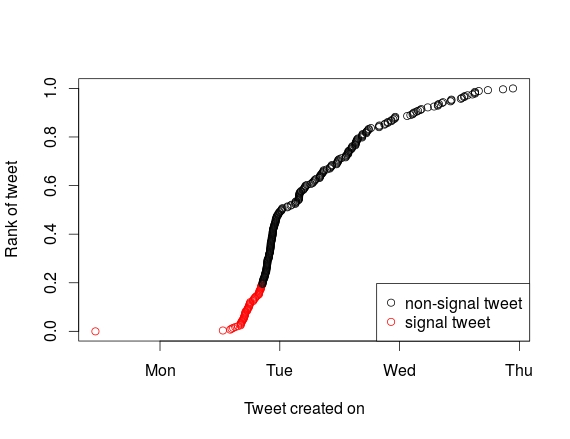
\includegraphics[width=\linewidth]{images/rumor1.jpeg}
		\captionof{figure}{Tweet Date vs Rank of Tweet - Example 1}
		\label{r1}
	\end{minipage}
	\hspace{.05\linewidth}
	\begin{minipage}{.45\linewidth}
		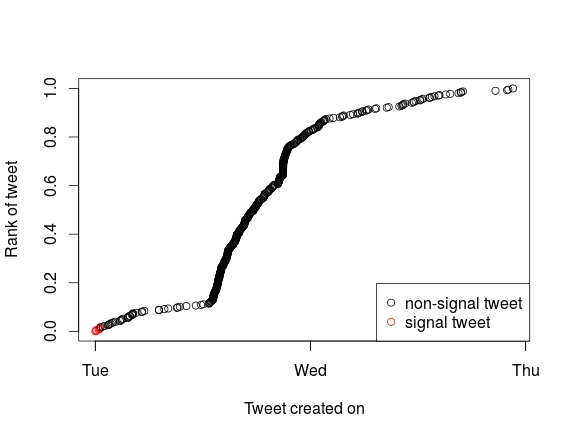
\includegraphics[width=\linewidth]{images/rumor2.jpeg}
		\captionof{figure}{Tweet Date vs Rank of Tweet - Example 2}
		\label{r2}
	\end{minipage}
	\centering
	\begin{minipage}{.45\linewidth}
		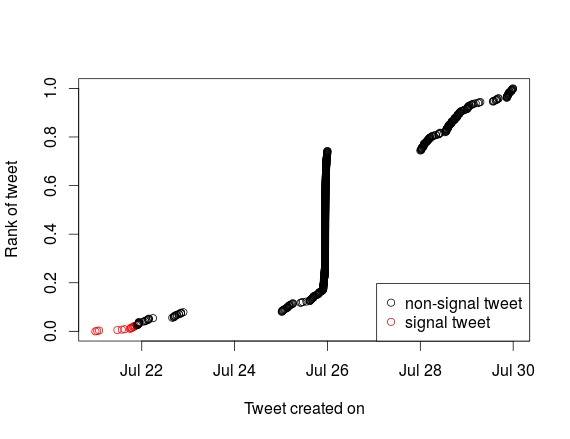
\includegraphics[width=\linewidth]{images/rumor3.jpeg}
		\captionof{figure}{Tweet Date vs Rank of Tweet - Example 3}
		\label{r3}
	\end{minipage}
	\hspace{.05\linewidth}
	\begin{minipage}{.45\linewidth}
		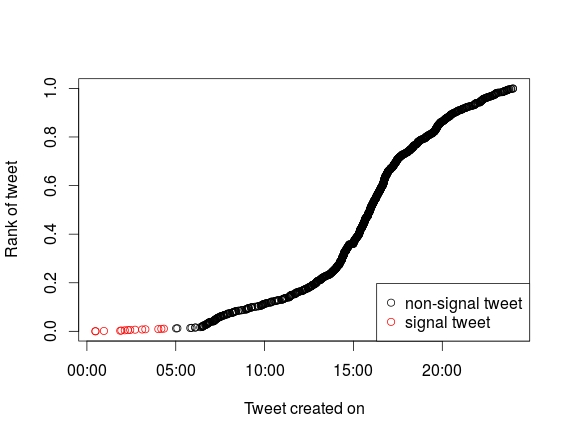
\includegraphics[width=\linewidth]{images/rumor4.jpeg}
		\captionof{figure}{Tweet Date vs Rank of Tweet - Example 4}
		\label{r4}
	\end{minipage}
\end{figure}



 
  In Figure \ref{r1} we plot the time of tweet v/s the rank of the tweet(i.e. sequence number of the tweet when ordered according to it's create time).It shows that the growth of a rumor is non-linear.We find different phases where the rumor starts to spread,then increases at a rapid rate and ultimately decaying after a certain point in time.Figure \ref{r2},\ref{r3} and \ref{r4} shows another similar instance of rumor growth rate.These different stages can be found by estimating the number of segments that are required to plot the curve.A rumor has many stages where rate of growth will be different at each stage thereby each of them resulting in a distinct segment on the plot.
 

 \section{Results - Burst Analysis }
 
 We now show the difference in burst patterns that are visible in rumors and non rumors.Here we divide the tweets in a rumor clusters in 30 bins divided by equal time intervals and plot the frequency of tweets in the corresponding bins.
 
 \begin{figure}[H]
 	\centering
 	\begin{minipage}{.45\linewidth}
 		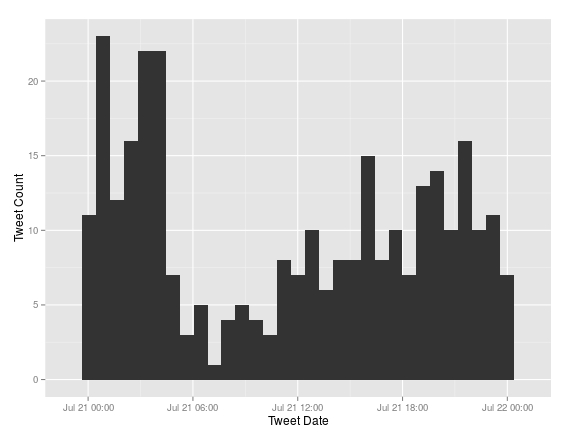
\includegraphics[width=\linewidth]{images/nrumorburst1.jpeg}
 		\captionof{figure}{Tweet Date vs Frequency - Example 1}
 		\label{nrb1}
 	\end{minipage}
 	\hspace{.05\linewidth}
 	\begin{minipage}{.45\linewidth}
 		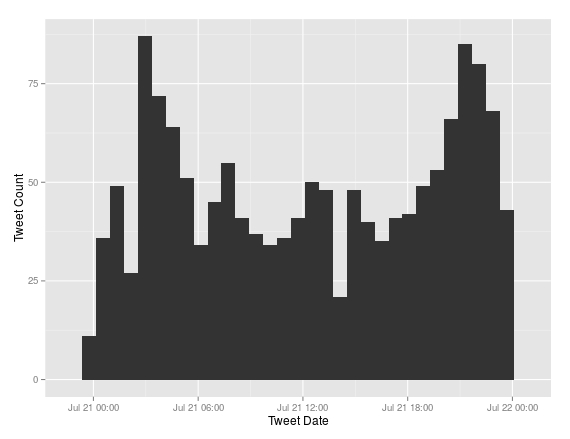
\includegraphics[width=\linewidth]{images/nrumorburst2.jpeg}
 		\captionof{figure}{Tweet Date vs Frequency - Example 2}
 		\label{nrb2}
 	\end{minipage}
 \end{figure}
 
  Figures \ref{nrb1} and \ref{nrb2} show the pattern observed in tweets which are non rumors.The distribution shows that number of tweets in every bin does not differ much.There is no presence of spikes in the plot which dominate every other bin in the plot.
 
  \begin{figure}[H]
  	\centering
  	\begin{minipage}{.45\linewidth}
  		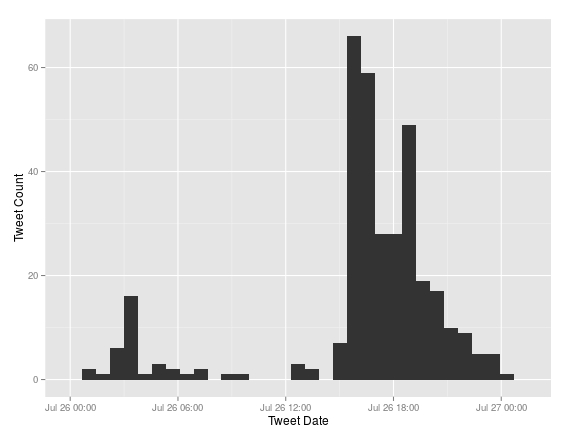
\includegraphics[width=\linewidth]{images/rumorburst1.jpeg}
  		\captionof{figure}{Tweet Date vs Frequency - Example 1}
  		\label{rb1}
  	\end{minipage}
  	\hspace{.05\linewidth}
  	\begin{minipage}{.45\linewidth}
  		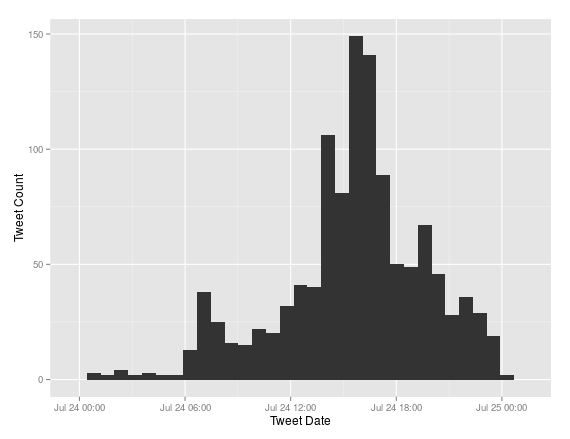
\includegraphics[width=\linewidth]{images/rumorburst3.jpeg}
  		\captionof{figure}{Tweet Date vs Frequency - Example 2}
  		\label{rb2}
  	\end{minipage}
  \end{figure}	
  
   Figures \ref{rb1} and \ref{rb2} show the pattern observed in tweets which are rumors.The distribution shows that number of tweets in every bin differs by a significant quantity.There exists at least one significant spike in the plot towards end of the plot when the rumor starts to become viral.Also,the initial bins seems to be less frequent as the rumor has still not propagated through a large number of users.
  	

\section{Results - Data Analysis }

  The following figures \ref{nrd1} and \ref{nrd2} show the Tweet Date vs Tweet Is-Signal scatter plot.We plot these values for all combinations of values of number of user mentions and number of hashtags thus resulting in several sub plots.
  The Tweet-Is-Signal property can have a value of 1 or 0 depending on whether the tweet contains enquiry patterns.
 
\begin{figure}[H]
	\centering
	\begin{minipage}{.7\linewidth}
		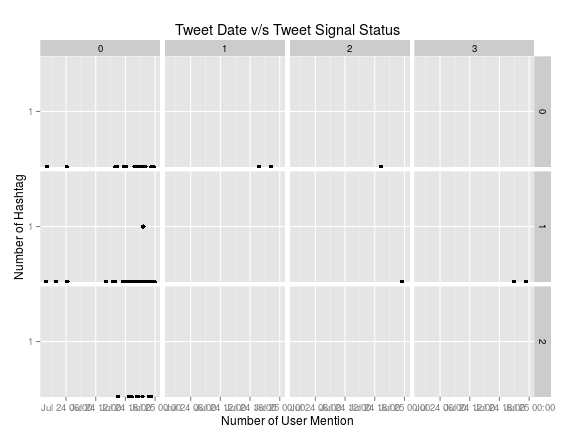
\includegraphics[width=\linewidth]{images/qp_nrumor1.jpeg}
		\captionof{figure}{Tweet Date vs Tweet-Is-Signal}
		\label{nrd1}
	\end{minipage}
\end{figure}

\begin{figure}[H]	
	\centering
	\begin{minipage}{.7\linewidth}
		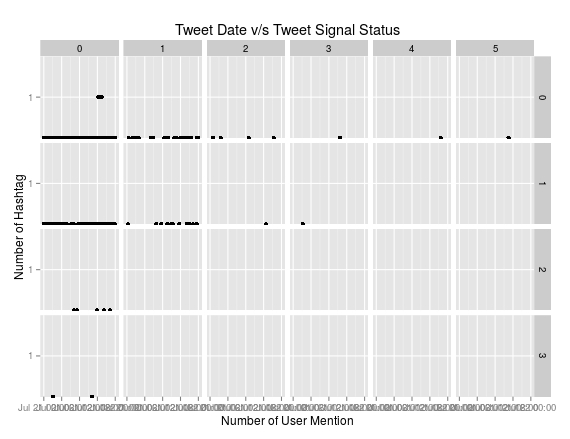
\includegraphics[width=\linewidth]{images/qp_nrumor2.jpeg}
		\captionof{figure}{Tweet Date vs Tweet-Is-Signal}
		\label{nrd2}
	\end{minipage}
\end{figure}

 Figures \ref{nrd1} and \ref{nrd2} show the behavior observed in tweet clusters that are non rumors.We see that signal tweets in such a case do not contain usermentions as well as hashtags except barring a few exceptions.

\begin{figure}[H]
	\centering
	\begin{minipage}{.7\linewidth}
		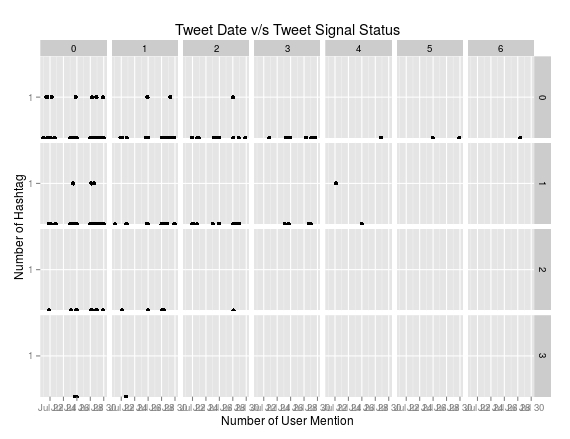
\includegraphics[width=\linewidth]{images/qp_rumor1.jpeg}
		\captionof{figure}{Tweet Date vs Tweet-Is-Signal}
		\label{rd1}
	\end{minipage}
\end{figure}
	
\begin{figure}[H]
	\centering
	\begin{minipage}{.7\linewidth}
		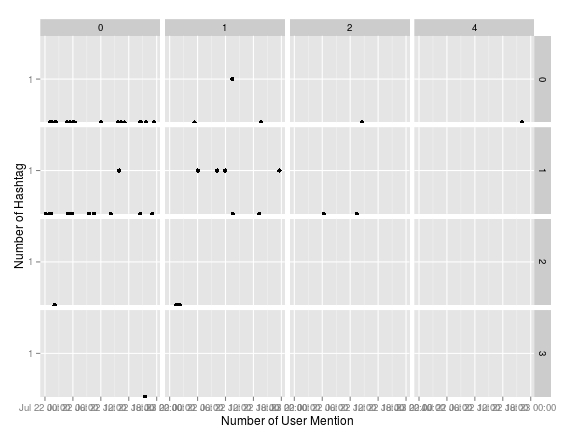
\includegraphics[width=\linewidth]{images/qp_rumor2.jpeg}
		\captionof{figure}{Tweet Date vs Tweet-Is-Signal}
		\label{rd2}
	\end{minipage}
\end{figure}

 Figures \ref{rd1} and \ref{rd2} show the behavior observed in tweet clusters that are rumors.We see that signal tweets in such a case  at least one contain user mentions or hashtags or a combination of both.
 
 \section{Summary}
 
 This chapter has focused on tweet clustering to accurately gather all tweets related to rumor.The dendrogram after initial clustering showed that clusters are not formed accurately due to sparse words in tweets and these clusters need to be combined further using another clustering algorithm.This helps in better prediction towards decision in the analysis part.The analysis part covered the difference in temporal and non-temporal properties of rumors which helps us to distinguish the both of them accurately.  	
% \newpage
% \chapter{Conclusion and Future Direction} 
This thesis described a system for automatic detection and verification of rumors about
real-world events on Twitter. Here we will summarize the contributions of this thesis and explore possible future directions for extending this work.
\section{Contribution of the Thesis}
The work described in this thesis describes how to create a system for detection and verification of rumors on Twitter.The major contributions are as follows:-
\begin{itemize}
\item We have used the NoSQL framework effectively to store the tweets given the huge volume of the tweets that are posted everyday.
\item The Hadoop framework has been effectively utilized to run the information retrieval algorithm given the size of the data involved for filtering and processing the necessary subset of tweets.
\item The extraction of semantic information to enrich the context of the rumor using Part-of-Speech tags
\item Extending the clustering algorithm of candidate rumor clusters for finding overlapping rumor clusters is a key component that has been developed.
\item A significant contribution of this thesis has been to find the essential temporal characteristics of the data and other Twitter specific meta data about tweets that constitute a rumor.
\end{itemize}
\clearpage
\section{Future scope}
There are many ways to extend the works presented in this thesis, several of which have been mentioned through out this document. Here, we will discuss what we believe to be
the the five most fruitful directions for future work. These directions are:
\begin{itemize}
	\item Linking to semantic web
	\item Design of classifier using temporal as well as non-temporal properties
	\item Extend system to other media platforms (social and traditional)
	\item Predict the impact of rumors
	\item Strategies for dampening the effects of rumors
\end{itemize}
	There are already a wide variety of linked data sources incorporated in the semantic web as mentioned in \cite{bontcheva2012making} .The main advantages of these data sources are that they provide plentiful amount of data on a growing number of topics and  they contain factual information about a large number of entities,covering these topics. The main goal is to exploit this semantic contextual information about entities contained in tweets by linking them to the data sources.This will aid in the data enrichment of the tweet data.Ultimately, this will help in the decision to identify rumors. 
    \\
    \par
    We have seen that the data properties of rumors and non rumors are different.The current work required manual intervention of looking at tweet content and verifying the same with the properties that the data exhibits.Using an exhaustive training data set which is annotated by an expert group of users who are trained to identify the correct rumors,we can build a classifier which will  automatically classify and therefore identify new rumors.
    \\
    \par	
	The current system is primarily designed for Twitter.Similar systems cam be extended for other social networks such as Facebook,Reddit and LinkedIn.Though some of the features described for this work are Twitter-specific,many of the features are platform-agnostic and can readily be extracted and processed from different platforms.
	\\
	\par
	In addition to detecting rumor,the system can predict the rate at which the rumor will spread and ultimately cease based on the recent data.This would be helpful to understand how many and up to what time people will be affected by the rumor.This is especially relevant for emergency services who might want to respond to false rumors that might have a large negative impact.
	\\
	\par
	Finally, a system that can detect rumors may be used as a tool to counter attack the spread of rumor by administering an "antidote" in the form of content which spreads verified information about the rumor.This again would be something that would have the most relevance to the emergency services dealing with real-world emergencies as they are the ones that have to deal with the consequences and the fallout of rumors on social media. 



\newpage

%============================ References ==============================

\bibliographystyle{ieetr}
\nocite{*} 
\bibliography{bibtex/1}


\end{document}
